\chapter{Generative Effects}

\exercise{1.1}
A function $f:\R\to\R$ is said to be
\begin{itemize}
    \item \emph{order-preserving} if $x \leq y$ implies $f(x) \leq f(y)$, for all $x, y \in \R$
    \item \emph{metric-preserving} if $|x-y|=|f(x)-f(y)|$
    \item \emph{addition-preserving} if $f(x+y)=f(x)+f(y)$
\end{itemize}
For each of the three properties defined above—call it \emph{foo}—find an $f$ that is \emph{foo}-preserving and an example of an $f$ that is not \emph{foo}-preserving.

\solution
$f(x) = x$ is order-, metric-, and addition-preserving.  $f(x) = x^2$ is none of these.

\exercise{1.4}
See book.

\solution
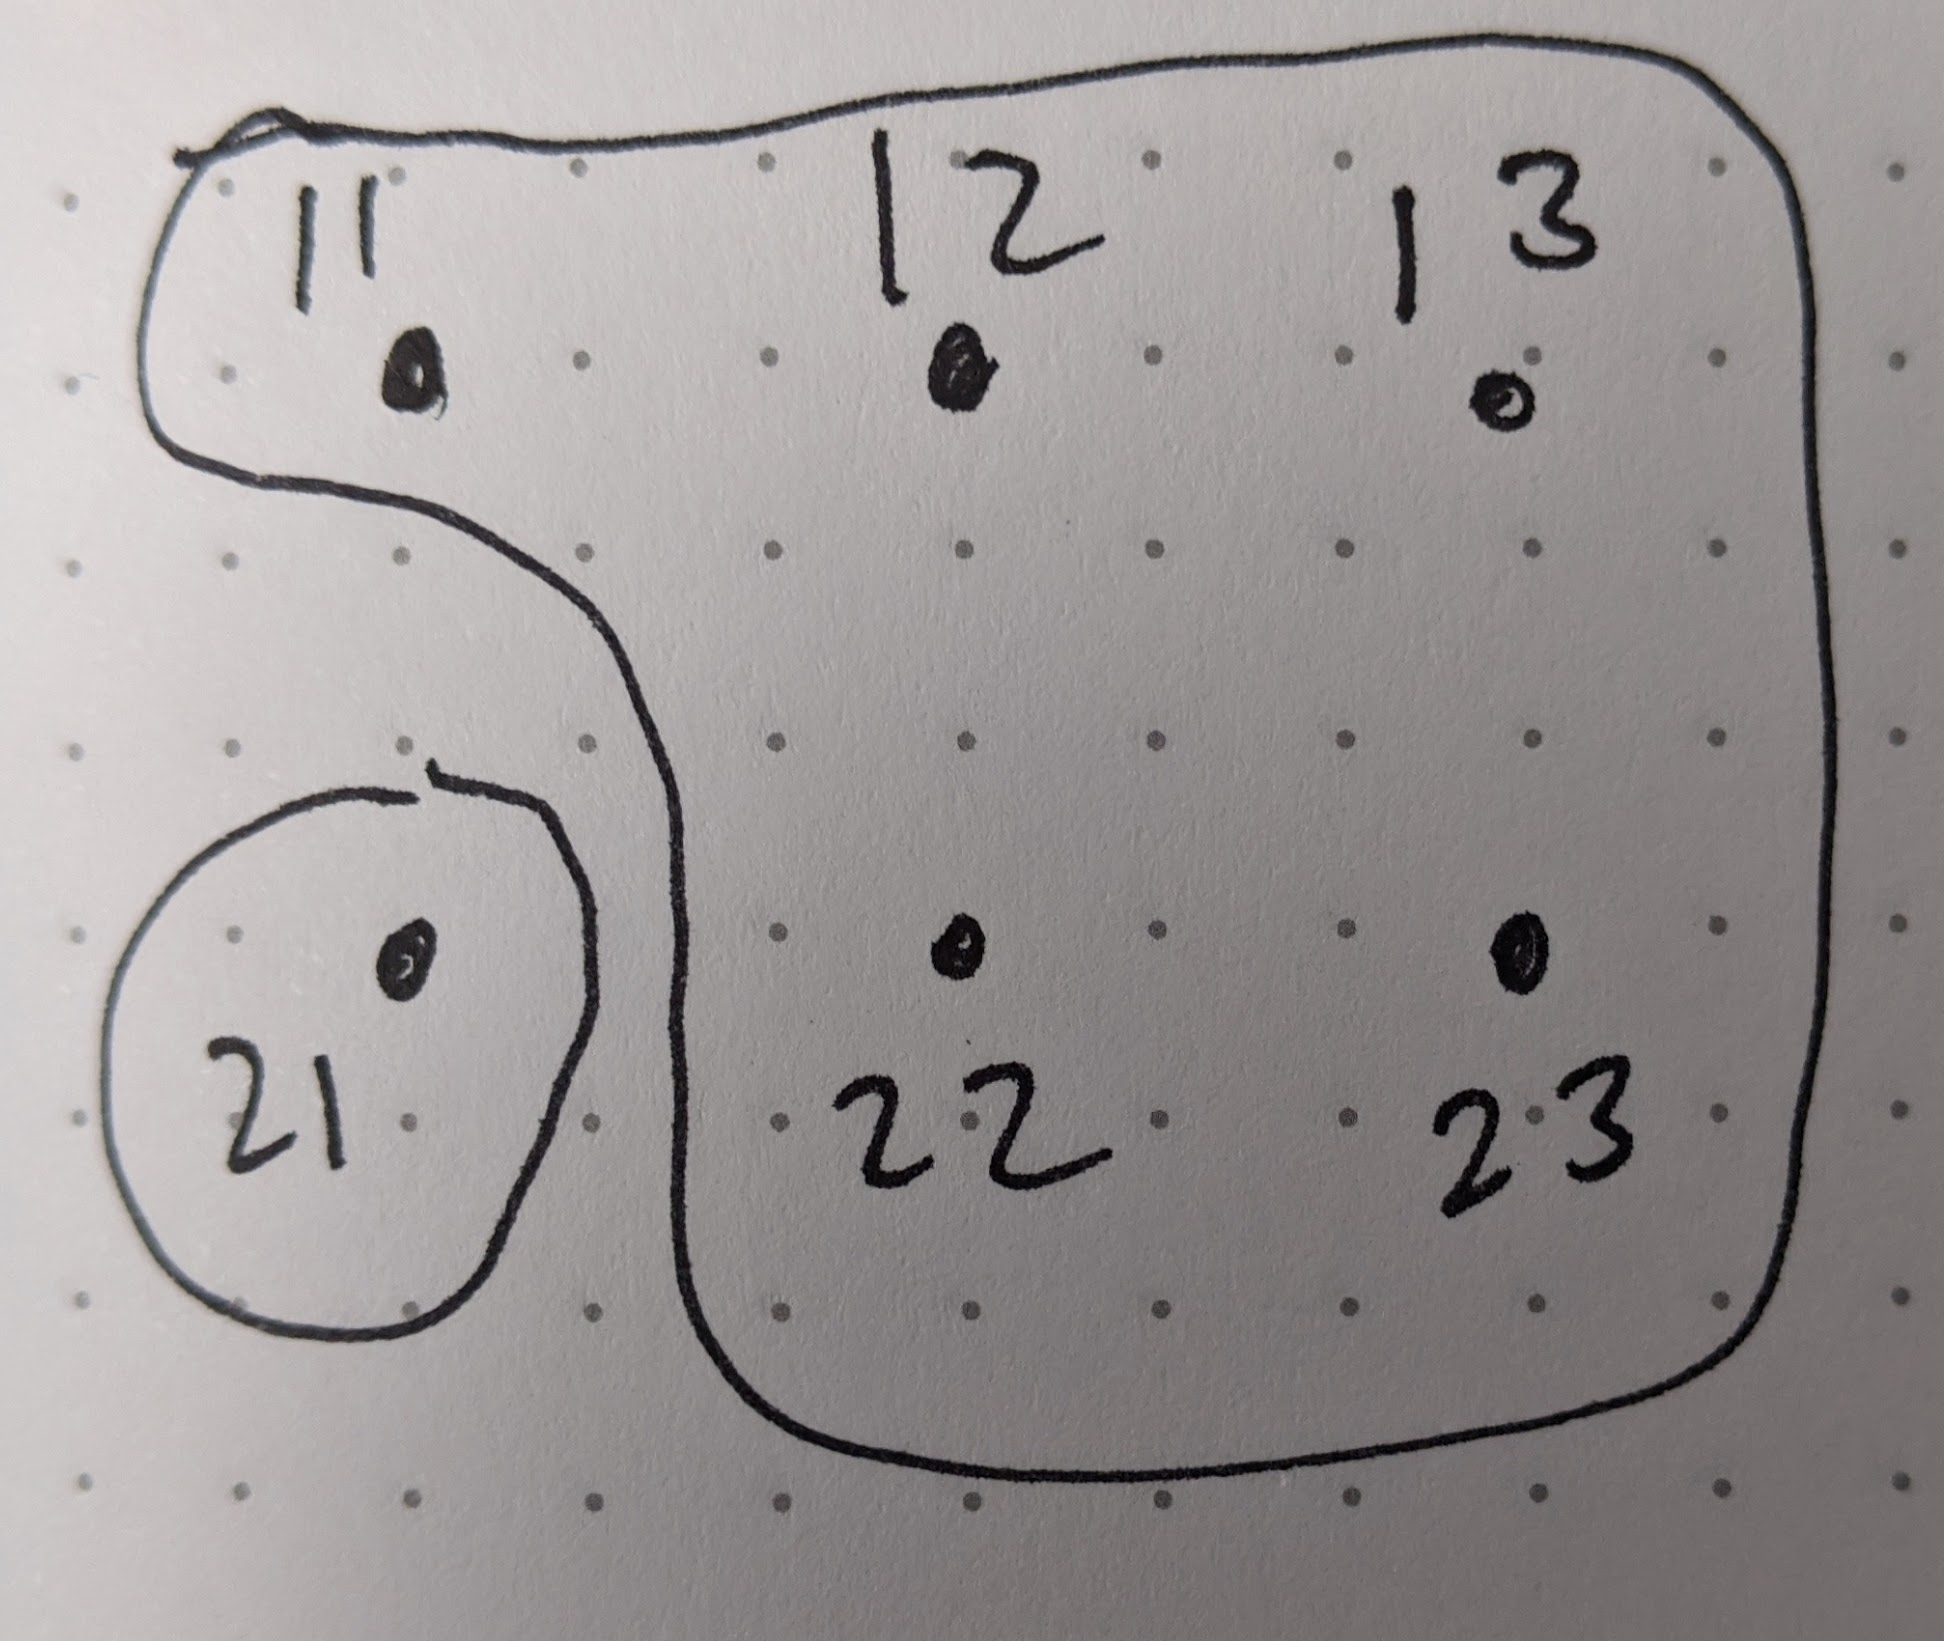
\includegraphics[width=0.5\linewidth]{images/1-4.jpg}

\exercise{1.6, 1.7, 1.10}
Discussed in person

\exercise{1.11}
Let $A = \{h, 1\}$ and $B = \{1, 2, 3\}$.

\solution
\begin{enumerate}
    \item The subsets of $B$ are $\varnothing, \{1\}, \{2\}, \{3\}, \{1, 2\}, \{1, 3\}, \{2, 3\}, \{1,2,3\}$.
    \item For example, $\{1, 2\} \cup \{2\} = \{1, 2\}$.
    \item $A\times B = \{(h, 1), (h, 2), (h, 3), (1, 1), (1, 2), (1, 3)\}$
    \item $A\sqcup B = \{h_A, 1_A, 1_B, 2_B, 3_B\}$
    \item $A\cup B = \{h, 1, 2, 3, 4\}$
\end{enumerate}

\exercise{1.16}
Suppose that $A$ is a set and $\{A_p\}_{p\in P}$ and $\{A'_{p'}\}_{p'\in P'}$ are two partitions of $A$ such that for each $p\in P$ there exists a $p'\in P'$ with $A_p = A'_{p'}$.
\begin{enumerate}
    \item Show that for each $p\in P$ there is at most one $p'\in P'$ such that $A_p= A'_{p'}$.
    \item Show that for each $p'\in P'$ there is a $p\in P$ such that $A_p = A'_{p'}$.
\end{enumerate}

\solution
\begin{enumerate}
    \item If there are distinct $p'_1, p'_2\in P'$ such that $A_p=A'_{p'_1}$ and $A_p=A'_{p'_2}$, then by transitivity $A'_{p'_1}=A'_{p'_2}$ which means that $p'_1=p'_2$ as $P'$ is a partition.
    \item Let $a\in A'_{p'_1}$.  Then we must have that $a\in A_p$ for some $p$.  We will show that this $A_p$ is the desired one.  There must exist $p'_2$ such that $A_p=A'_{p'_2}$.   So $a \in A'_{p'_2}$ and $a\in A'_{p'_1}$.  So $A'_{p'_1} = A'_{p'_2} = A_p$ as we wanted.
\end{enumerate}

\exercise{1.17}
See book.

\solution
$(11, 11), (12, 12), (13,13), (21,21), (22,22), (23,23), (11, 12), (12, 11), (22, 23), (23,22)$

\exercise{1.20}
Suppose that $\sim$ is an equivalence relation on a set $A$, and let $P$ be the set of $(\sim)$-closed and $(\sim)$-connected subsets $\{A_p\}_{p\in P}$.
\begin{enumerate}
    \item Show that each part $A_p$ is nonempty.
    \item Show that if $p\neq q$ i.e. $A_p \neq A_q$, then $A_p\cap A_q = \varnothing$.
    \item Show that $A = \bigcup_{p\in P} A_p$.
\end{enumerate}

\solution
\begin{enumerate}
    \item Since each $A_p$ is $(\sim)$-connected, by definition $A_p$ must be nonempty.
    \item Suppose $a\in A_p \cap A_q$. Then for any $b\in A_p$, we know $b\sim a$, hence since $A_q$ is $(\sim)$-closed we know $b\in A_q$.  Similarly for any $b\in A_q$.  Hence $A_p = A_q$.
    \item Clearly $\bigcup A_p\subseteq A$.  Suppose $a\in A$.  Then let $X=\{b\ |\ a\sim b, b\in A\}$.  $X$ is closed as the equivalence relation is reflexive and connected as it is transitive, so $X$ a set in $\{A_p\}$ and $A\subseteq \bigcup A_p$.
\end{enumerate}

\exercise{1.24}
Discussed in person

\exercise{1.25}
Suppose that $A$ is a set and $f : A \to\varnothing$  is a function to the empty set. Show that $A$ is empty.

\solution
Suppose there is some $a\in A$.  Then we must have $f(a)\in\varnothing$ which is clearly not possible.

\exercise{1.27, 1.38, 1.40, 1.41, 1.42, 1.44}
Discussed in person

\exercise{1.46}
Write down the numbers $1,2,\dots,10$ and draw an arrow $a\to b$ if $a$ divides perfectly into $b$. Is it a total order?

\solution
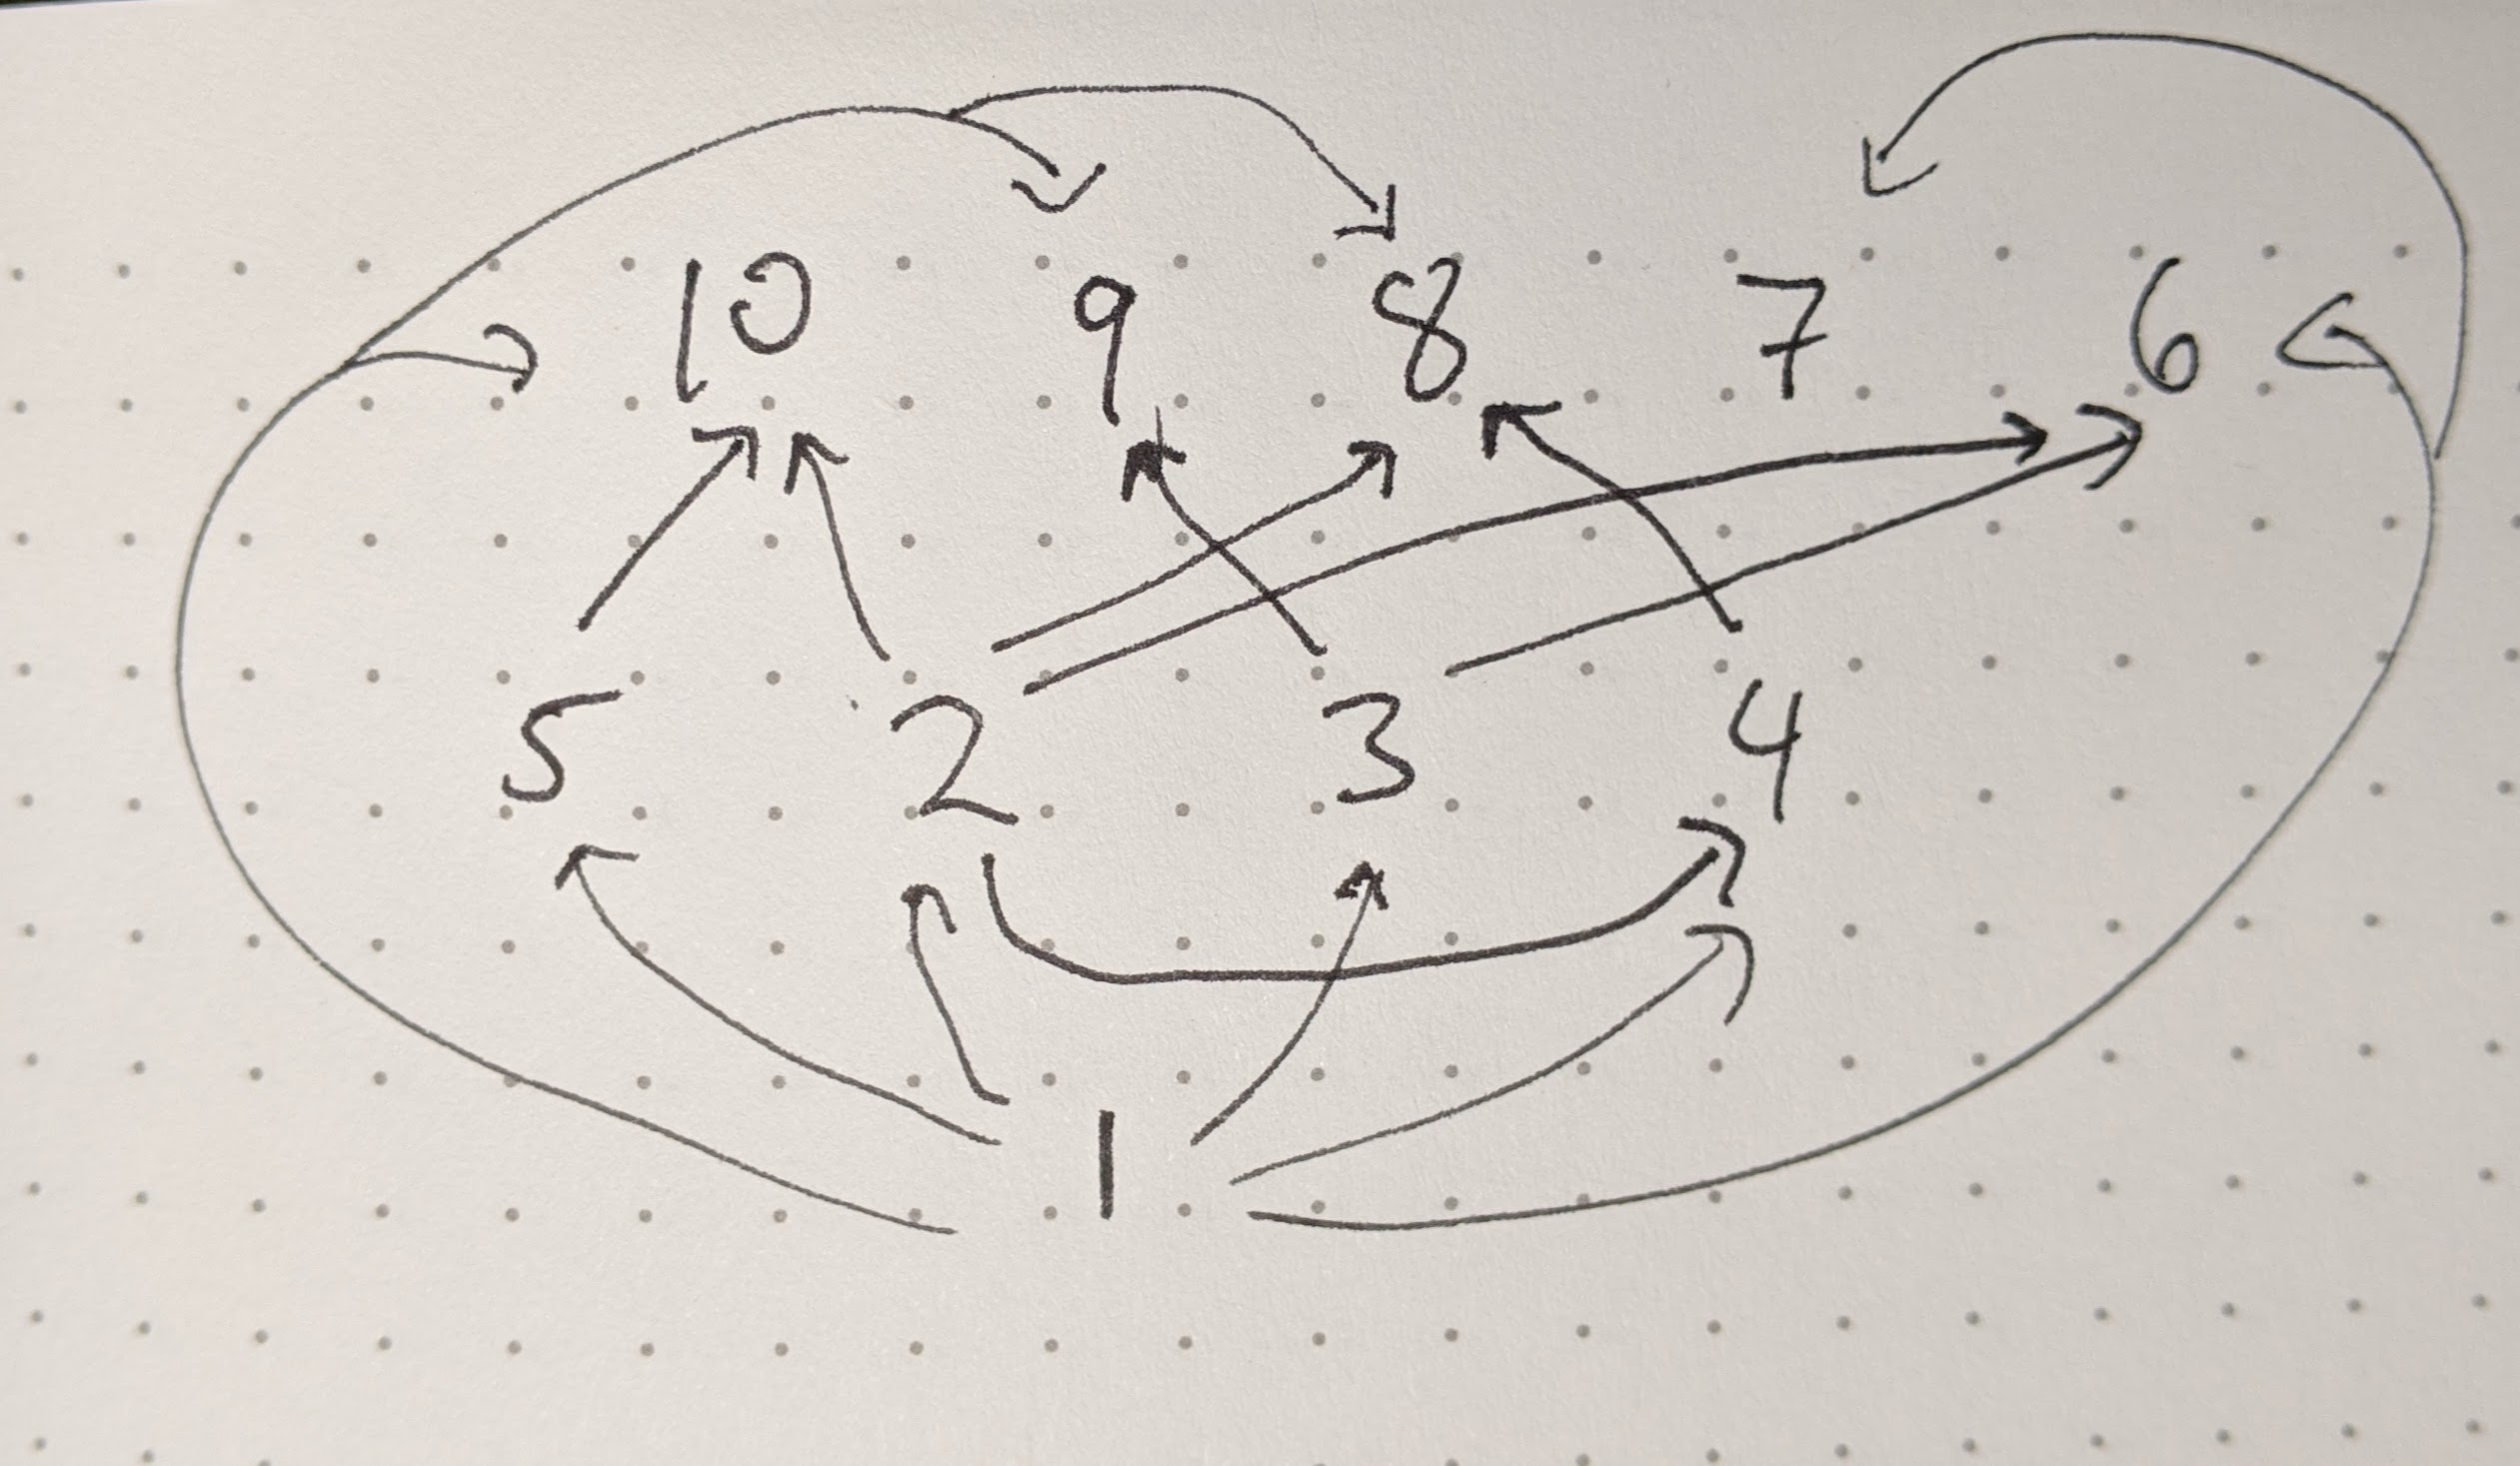
\includegraphics[width=0.5\linewidth]{images/1-46.jpg}

This isn't a total order, as for example we neither have $2|7$ or $7|2$.

\exercise{1.48}
Is the usual $\leq$ ordering on the set $\R$ of real numbers a total order?

\solution
Yes: for any $x,y\in\R$, we have $x\leq y$ or $y\leq x$.

\exercise{1.51}
Discussed in person

\exercise{1.53}
For any set $S$ there is a coarsest partition, having just one part. What surjective function does it correspond to?
There is also a finest partition, where everything is in its own partition. What surjective function does it correspond to?

\solution
Let $f:S\to\{\bullet\}$ be the unique function that sends every element of $S$ to $\bullet$.  This is a surjection corresponding to the coarsest partition, i.e. where every element is in the same set.

Let $f: S\to S$ be the identity function.  This is a surjection corresponding to the finest partition, i.e. where every element is in its own set.

\exercise{1.55}
Prove that the preorder of upper sets on a discrete preorder on a set $X$ is simply the power set $P(X)$.

\solution
Clearly the set of upper sets $U(X)$ is a subset of the power set $P(X)$.

Let $Y\subseteq X$.  We know $\varnothing$ is an upper set, so let $y\in Y$. Then since the preorder is discrete, the only element in $X$ greater than $y$ is y itself, which is in $Y$.  This holds for any $y\in Y$ so $Y$ is an upper set.  Note that the ordering on both $U(X)$ and $P(X)$ is the same, i.e. $\subseteq$.

\exercise{1.57}
See book.

\solution
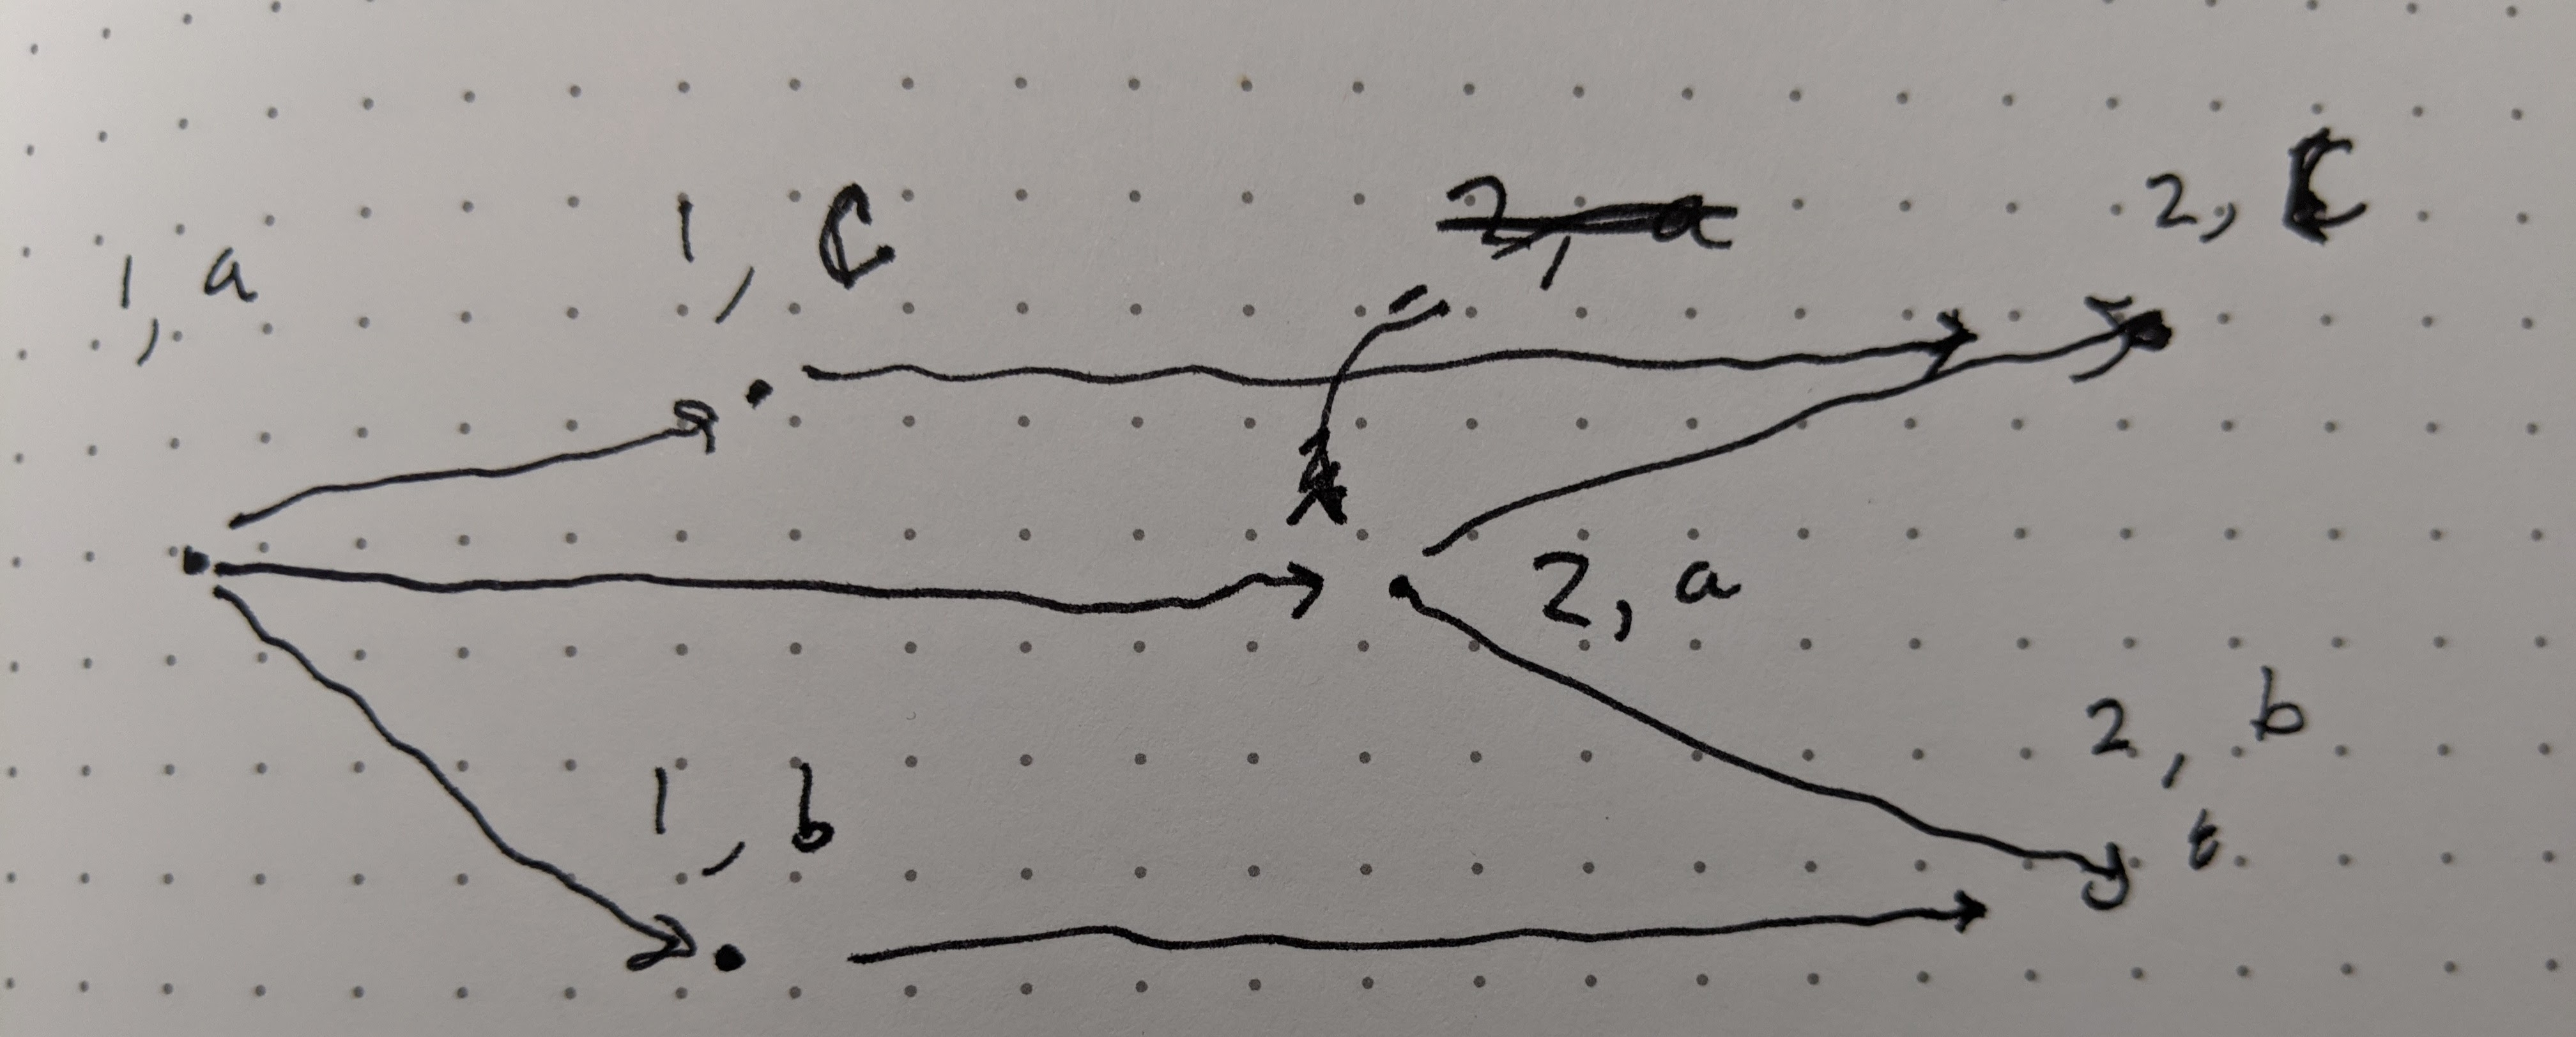
\includegraphics[width=0.5\linewidth]{images/1-57.jpg}

\exercise{1.63}
Let $X = \{0, 1, 2\}$.
\begin{enumerate}
    \item Draw the Hasse diagram for $P(X)$.
    \item Draw the Hasse diagram for the preorder $0 \leq 1 \leq 2 \leq 3$.
    \item Draw the cardinality map $|\cdot|$ as dashed lines between them
\end{enumerate}

\solution
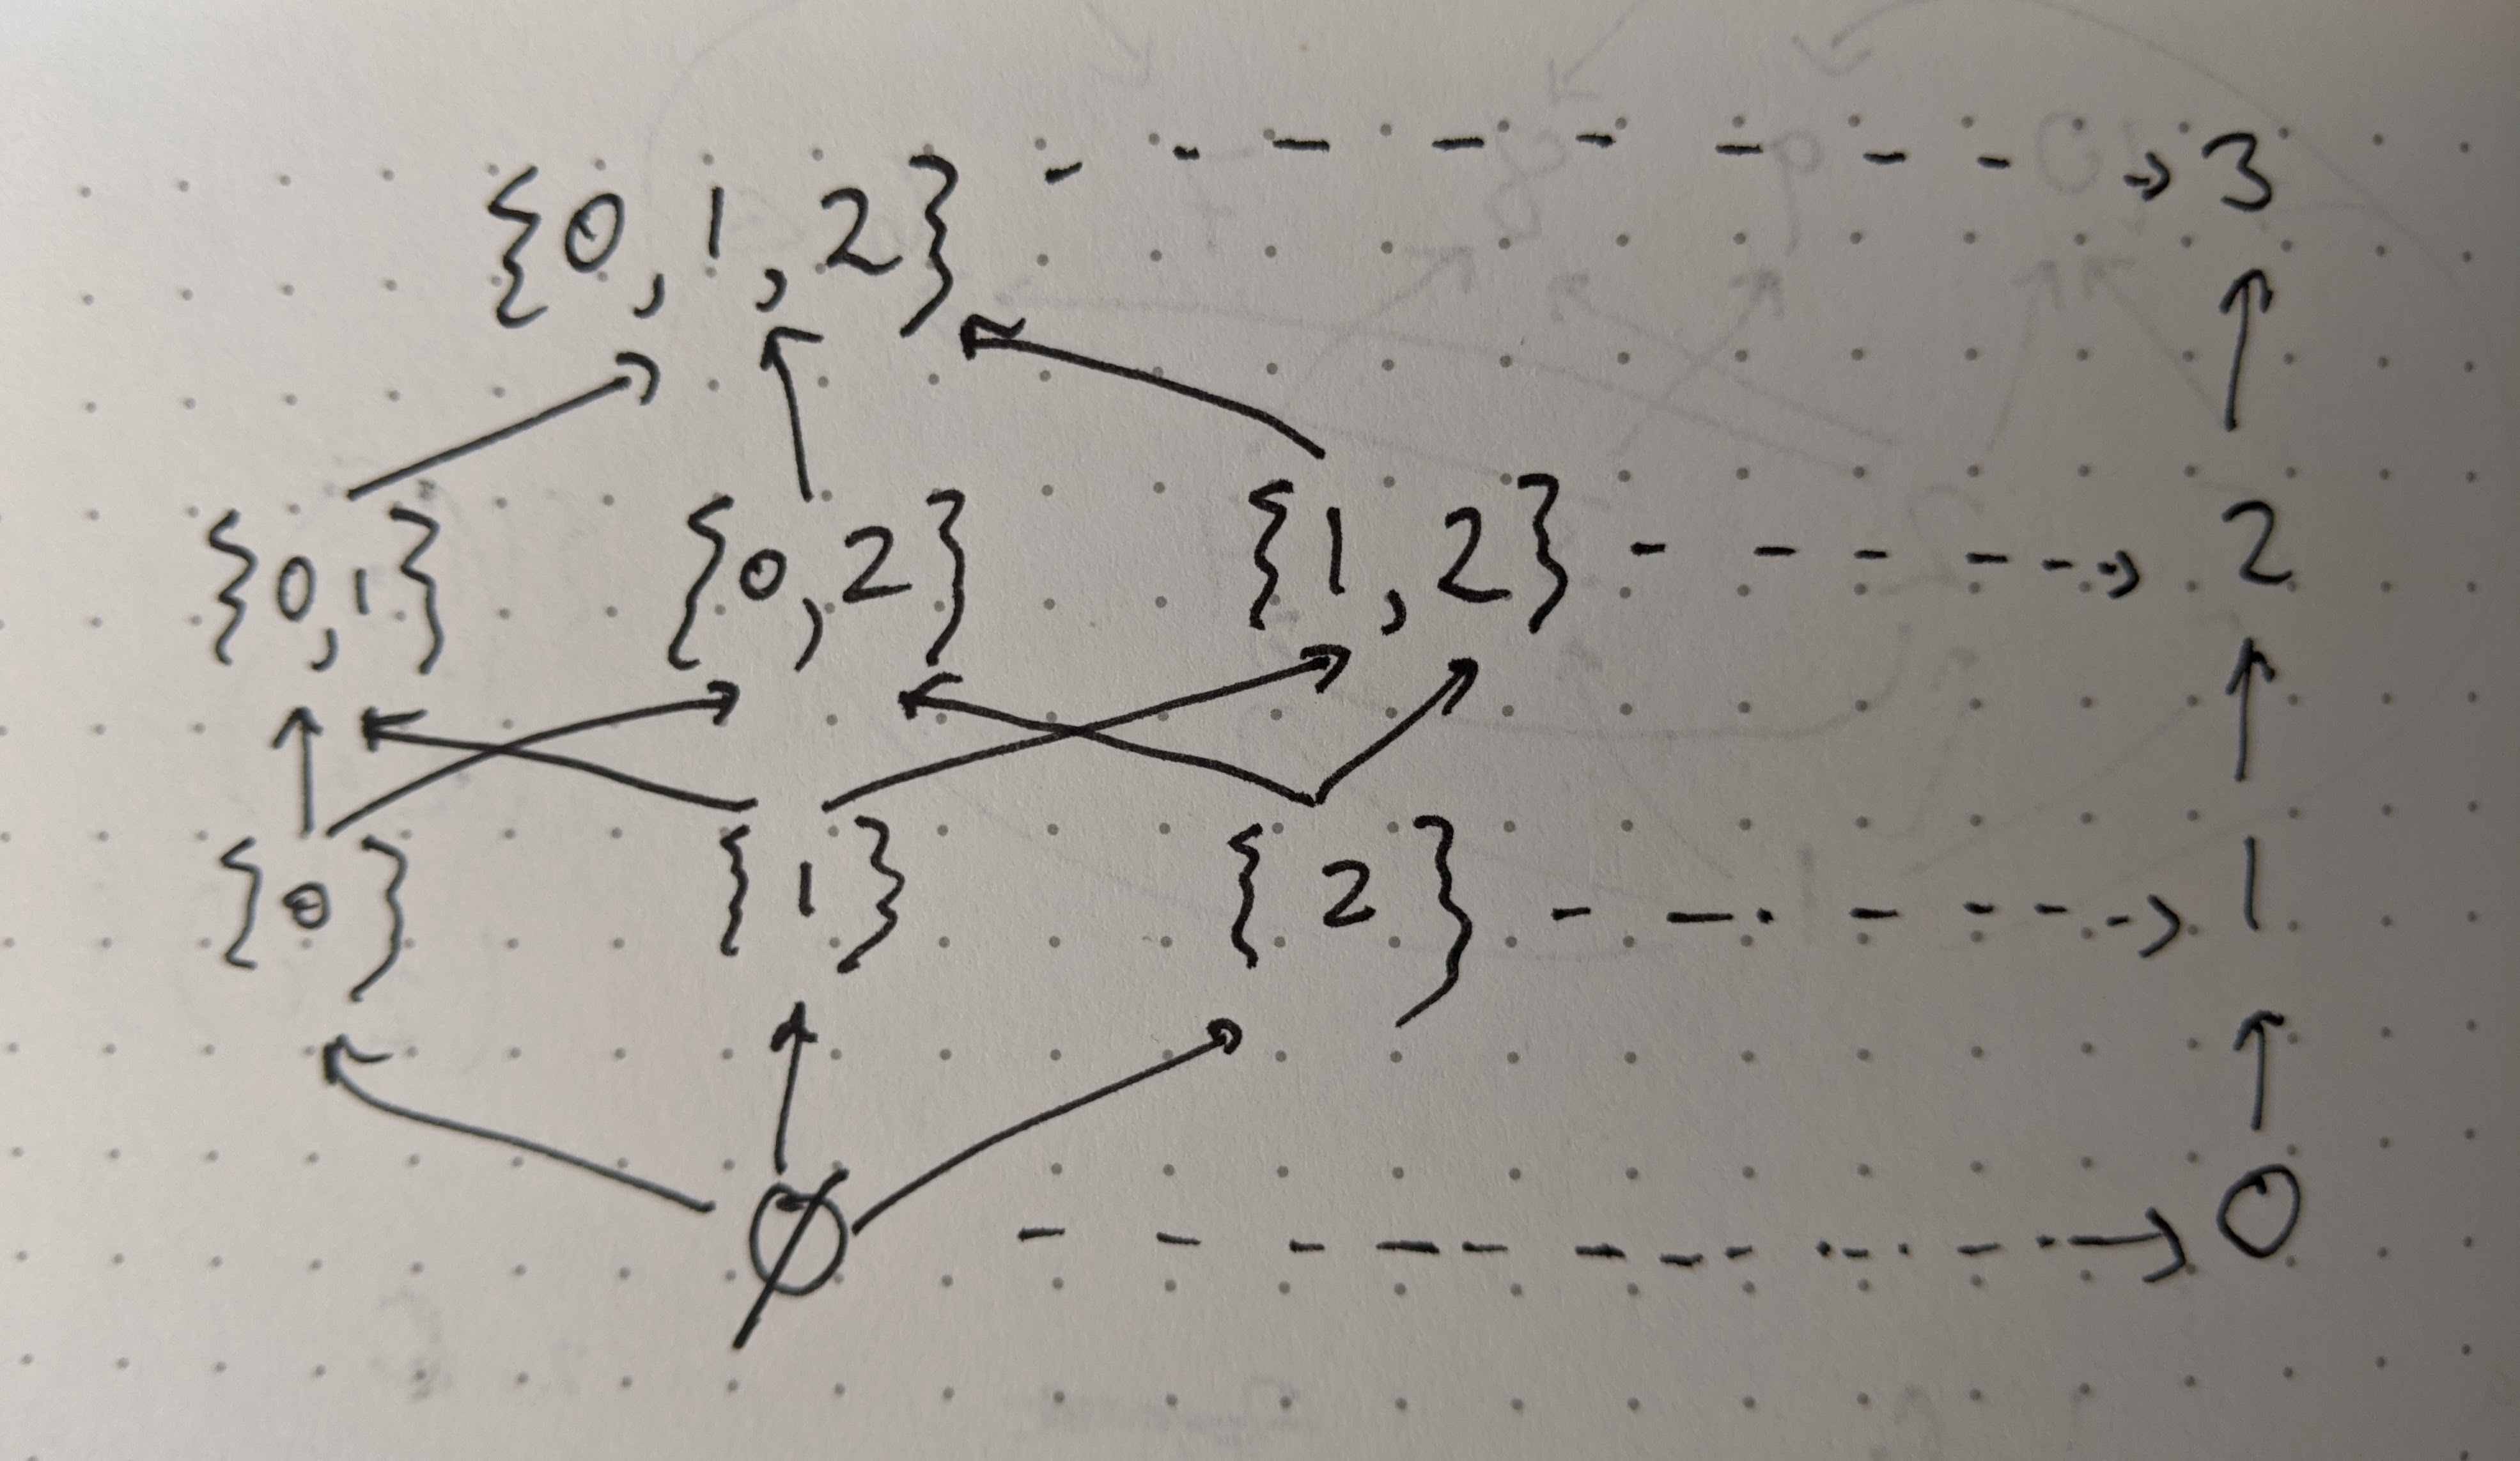
\includegraphics[width=0.5\linewidth]{images/1-63.jpg}

\exercise{1.65}
Draw the monotone map between $U(\B)$ and $P(\B)$ as described in the text.

\solution
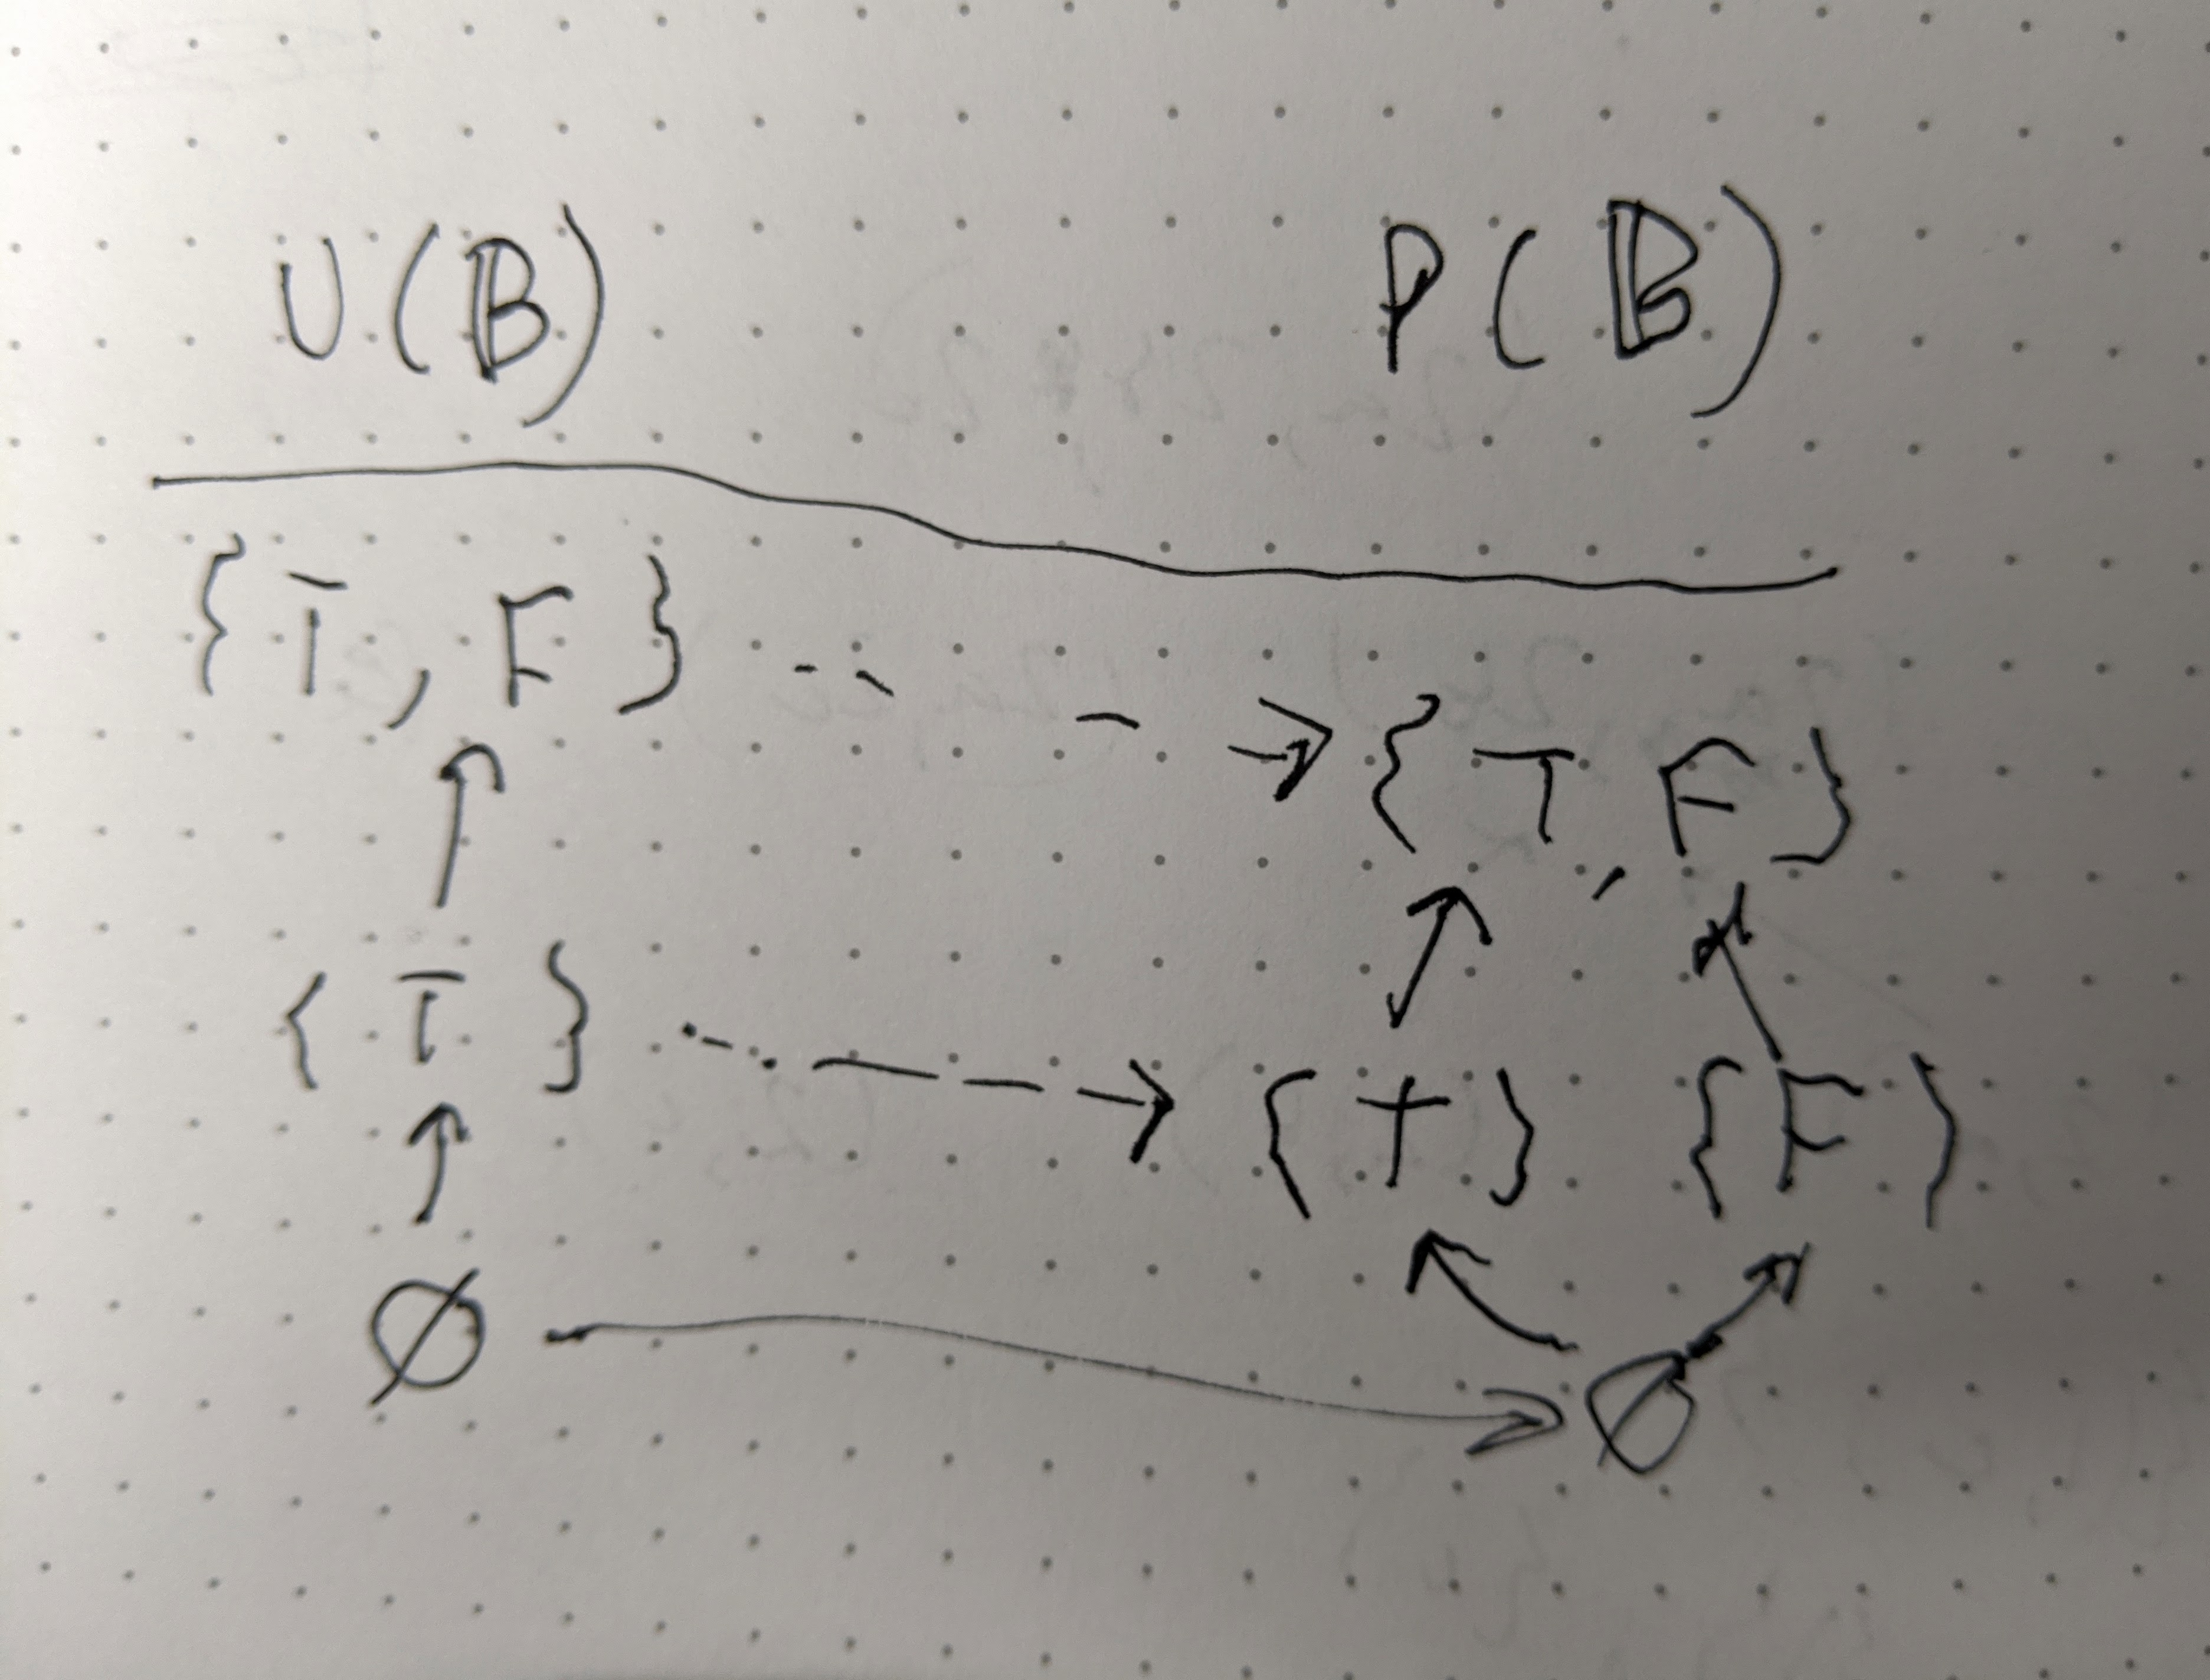
\includegraphics[width=0.5\linewidth]{images/1-65.jpg}

\exercise{1.66}
Let $(P, \leq)$ be a preorder.
\begin{enumerate}
    \item Show that the set $\uparrow p = \{p'\in P\ |\ p\leq p;\}$ is an upper set for any $p\in P$.
    \item Show that this defines a monotone map $\uparrow: P^{op}\to U(P)$.
    \item Show that $p\leq p'$ iff $\uparrow(p')\subseteq\uparrow(p)$.
    \item Draw a picture of the map $\uparrow$ in the case where $P$ is the preorder $(b\geq a\leq c)$.
\end{enumerate}

\solution
\begin{enumerate}
    \item Suppose $q\in \uparrow p$, then any $q'\geq q$ is transitively greater than $p$ and hence $q'\in \uparrow p$.
    \item Suppose $p\geq q$ (i.e. $p$ is less than $q$ in $P^{op}$), we want to show that $\uparrow p \subseteq \uparrow q$.  So let $p'\in \uparrow p$.  We know $q\leq p\leq p'$ and hence $p'\in\uparrow q$.
    \item We showed the first direction in part 2, so assume $\uparrow(p')\subseteq \uparrow(p)$.  This means $p\in \uparrow(p')$ and hence $p\leq p'$.
    \item 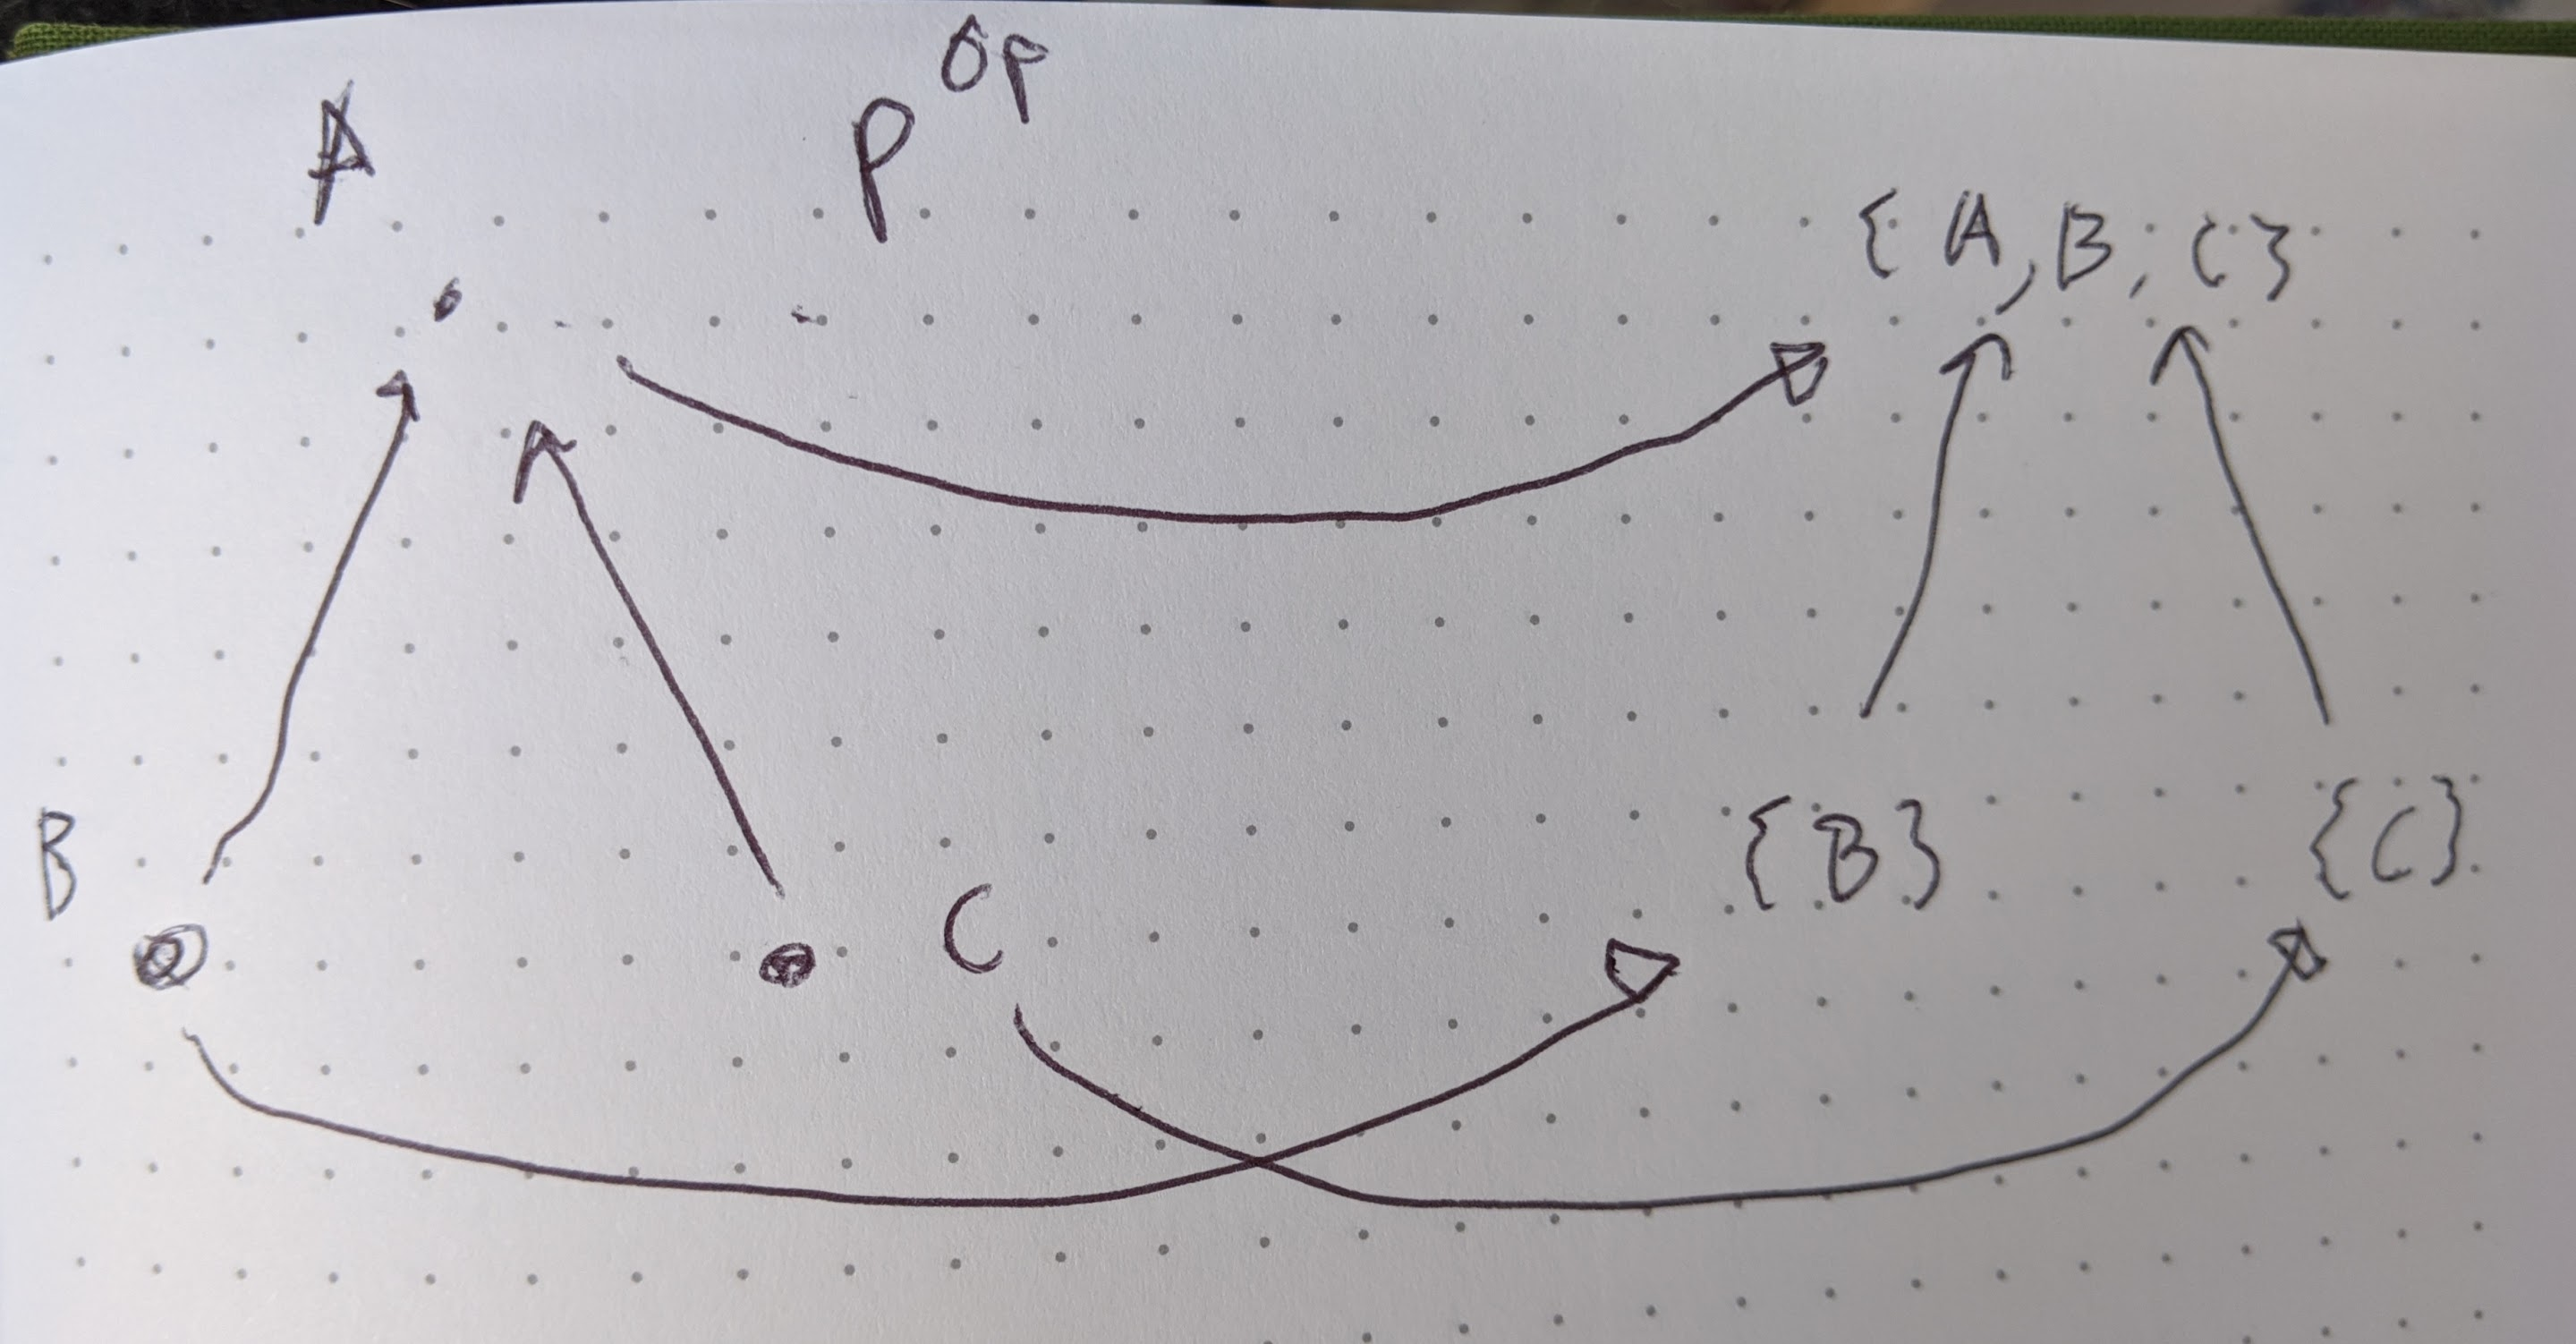
\includegraphics[width=0.5\textwidth]{images/1-66.jpg}
\end{enumerate}

\exercise{1.67}
Show that when $(P, \leq_P)$ is a discrete preorder, then every function $f:P\to Q$ is monotone regardless of the order $\leq_Q$.

\solution
We need to show that for any $x,y\in P$ where $x\leq_P y$, we have $f(x)\leq_Q f(y)$.  But the only $x$ and $y$ satisfying this are $x\leq_P x$, for which we have $f(x)\leq_Q f(x)$ regardless of $\leq_Q$ by the definition of a preorder.

\exercise{1.69}
Choose two sets $X$ and $Y$ with at least three elements each and choose a surjective, non-identity function $f:X\to Y$.  Write down two different partitions $P$ and $Q$ of $Y$, and find $f^*(P)$ and $f^*(Q)$.

\solution
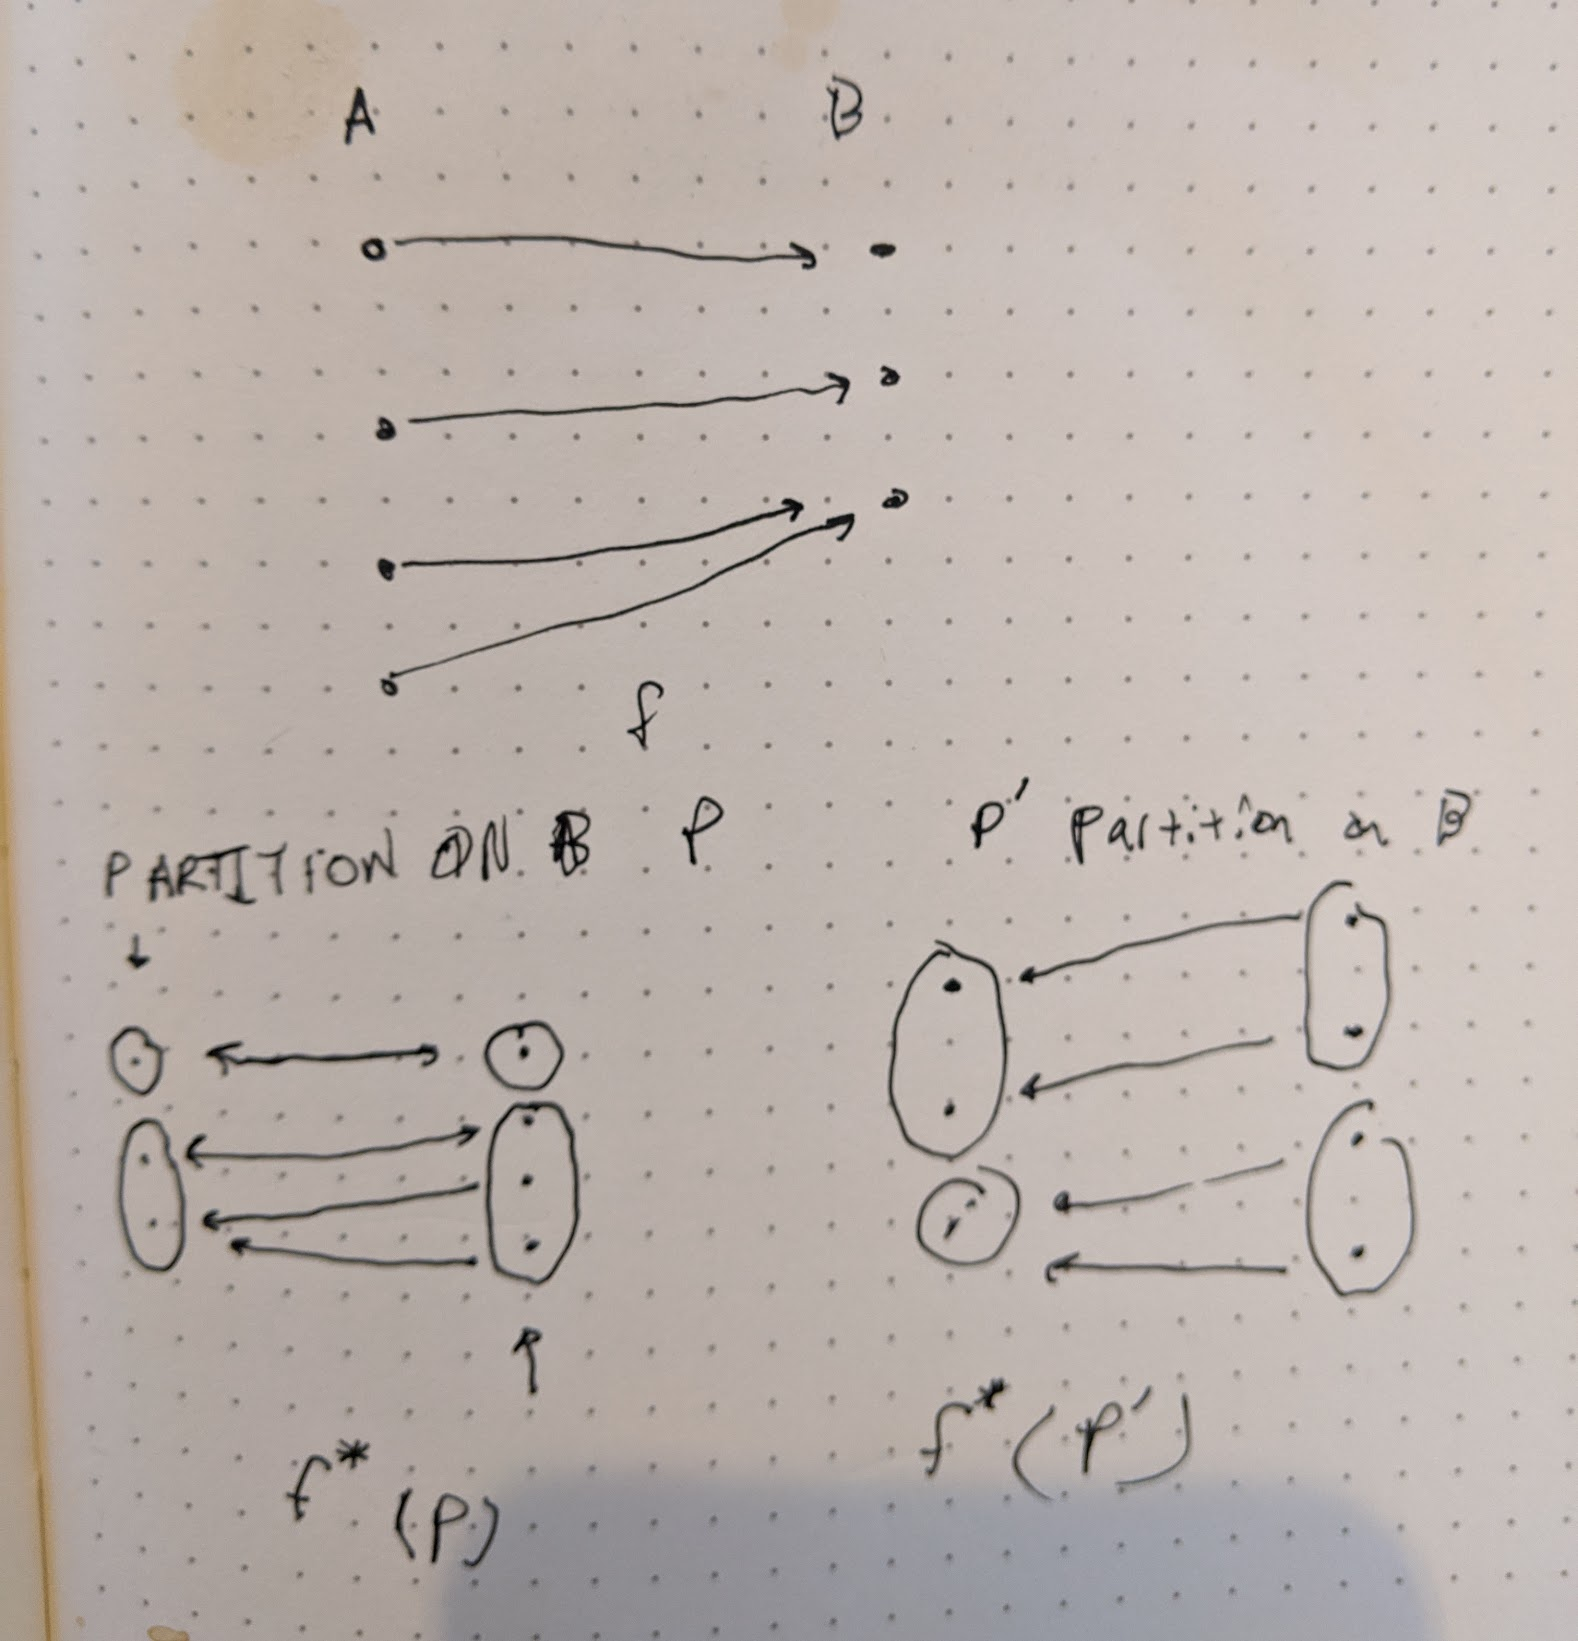
\includegraphics[width=0.5\linewidth]{images/1-69.jpg}

\exercise{1.71}
Prove Proposition 1.70:
\begin{enumerate}
    \item For any preorder $(P, \leq_P)$, the identity function is monotone.
    \item If $(Q, \leq_Q)$ and $(R, \leq_R)$ are preorders and $f:P\to Q$ and $g:Q\to R$ are monotone, then $(f\fcmp g):P\to R$ is also monotone.
\end{enumerate}

\solution
\begin{enumerate}
	\item If $a \leq_P b$ then clearly $a = f(a)\leq_P f(b) = b$ if $f$ is the identity function.
	\item Suppose $a\leq_P b$, then $f(a) \leq_Q f(b)$ as $f$ is monotone, and hence $g(f(a)) \leq_R g(f(b))$ as $g$ is also monotone.
\end{enumerate}

\exercise{1.73}
Show that a skeletal dagger preorder is just a discrete preorder, and hence can be identified with a set.

\solution
Let $(P, \leq)$ be a skeletal dagger preorder.  We need to show that for any $x\in P$, the only thing comparable to $x$ is $x$ itself.  So suppose $x\leq y$, then as $P$ is a dagger preorder we know that $y\leq x$.  Hence as $P$ is skeletal, we have that $x=y$.  This implies that $P$ is a discrete preorder.

\exercise{1.77}
Show that the map $\Phi$ from Section 1.1.1 (`Is $\bullet$ connected to $\star$?') is the monotone map $Prt(\{\star, \bullet, \circ\})\to\B$.

\solution
Let $P$ and $P'$ be partitions where $P\leq P'$.  If $\Phi(P)=\texttt{false}$ then clearly $\Phi(P)\leq\Phi(P')$, so assume $\Phi(P) = \texttt{true}$.  This means for some set $X$ in the partition $P$, we know that both $\bullet, \star\in X$.  As $P\leq P'$ this means there is some $Y$ in the partition $P'$  with $X\subseteq Y$, which implies that $\bullet,\star\in Y$.  Hence $\Phi(P')=\texttt{true}$ and $\Phi(P)\leq\Phi(P')$.

\exercise{1.79}
Let $P$ and $Q$ be preorders and $f:P\to Q$ a monotone map.  Show that the pullback $f^*:U(Q)\to U(P)$ can be defined by taking $u:Q\to\B$ to $(f\fcmp u):P\to\B$.

\solution
Call $\phi_Q$ the function that takes upper sets in $Q$ to monotone maps as defined in Proposition 1.78, and similarly $\phi_P$.  Let $U\in U(Q)$.  We want to show $\phi_P(f^{-1}(U)) = f\fcmp (\phi_Q(U))$.

Let $x\in P$.  If $x\in f^{-1}(U)$, then we know $\phi_P(f^{-1}(U))(x)=\texttt{true}$ by definition.  But we also know $f(x)\in U$ and hence $\phi_Q(U)(f(x)) = \texttt{true}$.  Conversely if $x\not\in f^{-1}(U)$, we will have both $\phi_P(f^{-1}(U))(x)=\texttt{false}$, as well as $f(x)\not\in U$ and $\phi_Q(U)(f(x)) = \texttt{false}$.  This shows that these maps are equal.

\exercise{1.80}
Why is 0 a greatest lower bound for $\left\{\frac{1}{n+1}\ |\ n\in\N\right\}\subseteq\R$?

\solution
Assume that $\varepsilon > 0$ is a lower bound. Let $n=\lceil 1 / \varepsilon \rceil$.  Then
\[
	\frac{1}{n+1}\leq \frac{1}{1 / \varepsilon +1} \leq \frac{1}{1/\varepsilon}=\varepsilon.
\]
Hence no such $\varepsilon$ is a lower bound.

\exercise{1.85}
Let $(P, \leq)$ be a preorder and $p\in P$, consider the set $A=\{p\}$.
\begin{enumerate}
	\item Show that $\bigwedge A \cong p$.
	\item Show that if $P$ is a partial order, then $\bigwedge A = p$.
	\item Are the analogous facts true when $\bigwedge$ is replaced by $\bigvee$?
\end{enumerate}

\solution
\begin{enumerate}
	\item Clearly $p\leq p$, so by definition $\bigwedge A \leq p$ (as a lower bound) and $\bigwedge A\geq p$ (as a greatest lower bound).
	\item If the previous is true in a partial order, then we have $\bigwedge A = p$.
	\item The analogous facts are true with $\bigvee$.
\end{enumerate}

\exercise{1.90}
In the $n|m$ ordering on $\N$, what are the meet and the join?

\solution
The meet is the greatest common divisor and the join is the least common multiple.

\exercise{1.94}
Prove that for any monotone map $f:P\to Q$, if $a, b\in P$ have a join and $f(a), f(b)\in Q$ have a join, then $f(a)\lor f(b)\leq f(a\lor b)$.

\solution
We know $a,b\leq a\lor b$, so since $f$ is monotone we have $f(a), f(b)\leq f(a\lor b)$.  Hence $f(a\lor b)$ is an upper bound for $\{f(a), f(b)\}$, so by definition of the join we must have $f(a)\lor f(b)\leq f(a\lor b)$.

\exercise{1.98}
Find a right adjoint for the monotone map $(3\times -):\Z\to\R$, and show it is correct.

\solution
Let $g(y) = \lfloor y/3 \rfloor$.  Then we have $3x \leq y \iff x\leq y/3 \iff x\leq \lfloor y/3\rfloor$, hence $g$ is a right adjoint for $3x$.

\exercise{1.99}
See book.

\solution
\begin{enumerate}
	\item In this case $f$ is left adjoint to $g$.
	\item In this case $f$ is not left adjoint to $g$, as $g(1)=2\geq 2$ but $f(2)=2\nleq 1$.
\end{enumerate}

\exercise{1.101}
\begin{enumerate}
	\item Does $\lceil -/3\rceil$ have a left adjoint $L:\Z\to\R$?
	\item If not, why?  If so, does its left adjoint have a left adjoint?
\end{enumerate}

\solution
Let $g:\R\to\Z$ be defined by $g(x)=\lceil x/3 \rceil$.  We will show by contradiction that $g$ does not have a left adjoint.

For a left adjoint $f:\Z\to\R$, we must have $f(1)\leq 0 \iff 1\leq g(0)=\lceil 0/3\rceil=0$.  Clearly the second part does not hold, so we know $f(1)\nleq 0$.

On the other hand, we know that $f(1)\leq \inf A$ where $A=\{x | g(x)\geq 1, x\in\R\}$.  However $1/n\in A$ for $n\in\Z^+$, as $\lceil 1/n\rceil = 1$ for all such $n$.  But $\inf\{1/n | n\in\Z^+\}=0$, which implies that $f(1)\leq 0$.  This is a contradiction, so $g$ must not have a left adjoint.

\exercise{1.103}
Choose 6 different partitions on the set $S$ and for each, call it $c$, find $g_!(c)$ where $S, T,$ and $g:S\to T$ are the same as they were in Example 1.102.

\exercise{1.105}
Using the same $S, T,$ and $g:S\to T$ as in Example 1.102, find the partition $g^*(c)$ for each of the 5 partitions $c$ on the set $T$.

\solution
For both 1.103 and 1.105.

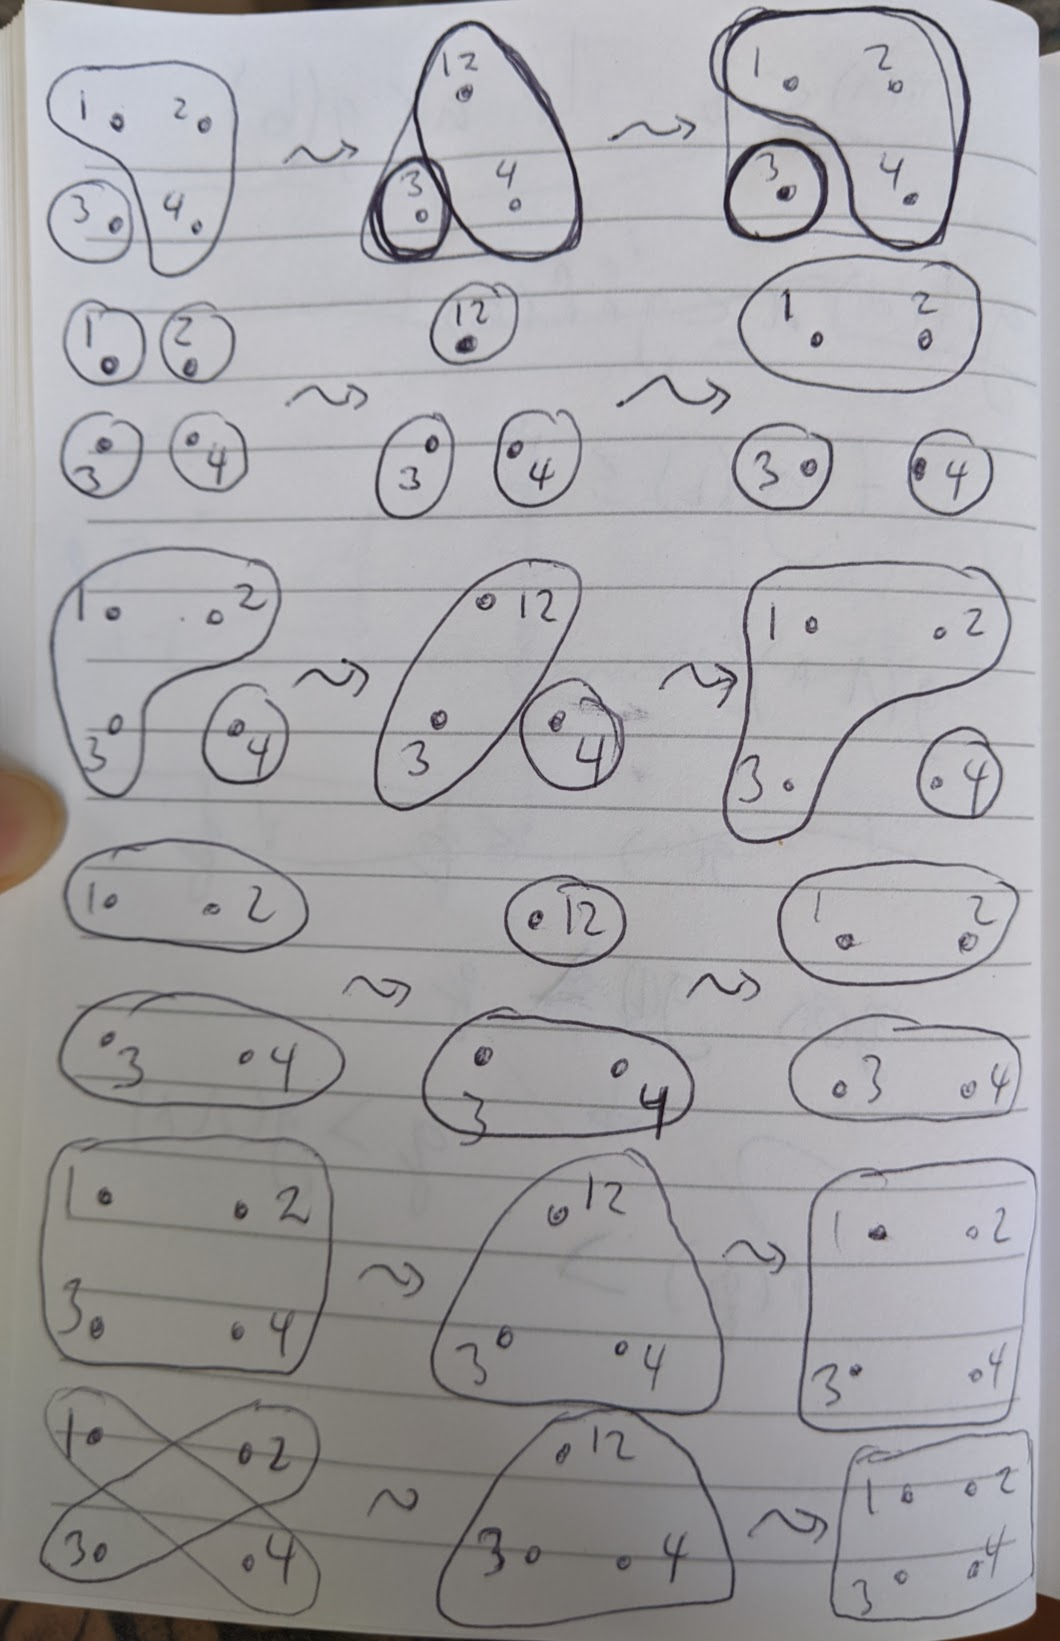
\includegraphics[width=0.5\linewidth]{images/1-105.jpg}

\exercise{1.106 (revised)}
Prove that $g_!$ is left adjoint to $g^*$, as defined in the text.
%Let $S,T,$ and $g:S\to T$ be as in Example 1.102.
%\begin{enumerate}
%	\item Choose a nontrivial partition $c:S\to P$ and let $g_!(c)$ be its push forwards partition on $T$.
%	\item Choose any coarser partition $d:T\to P'$, i.e. where $g_!(c)\leq d$.
%	\item Choose any non-coarser partition $e:T\to Q$, i.e. where $g_!(c)\nleq e$.
%	\item Find $g^*(d)$ and $g^*(e)$.
%	\item Since $g_!(c)\leq d$ and $g_!(c)\nleq e$, we should have $c\leq g^*(d)$ and $c\nleq g^*(e)$.  Show that this is true.
%\end{enumerate}

\solution

Let $S, T$ be sets, and let $g: S \to T$.  Define $g_{!}, g^{*}$ as in the text.  

We first show $g^{*}$ is monotone.  Let $A, B\in Prt(T)$ such that $A\leq B$.  Then for each set $A_i\in A$, $A_i \subseteq B_j$ for some $B_j\in B$, and as a result $g^{-1}(A_i)\subseteq g^{-1}(B_j)$ for each $A_i\in A$.  As the image of a partition under $g^*$ is the collection of preimages of that partition via $g$, we have $g^{*}(A)\leq g^{*}(B)$.

Next we show $g_!$ is monotone.  Let $A, B\in Prt(S)$ such that $A\leq B$.  As before we know that for each set $A_i\in A$, $A_i\subseteq B_j$ for some $B_j\in B$. We consider $A,B\in Rel(S)$ i.e. subsets of $S\times S$. Note that $g_{!}(C)$  is the transitive closure of the relation $\{ (g(x),g(y)| (x, y)\in C\}$.  As $A\leq B$, $\{ (g(x),g(y)| (x, y)\in A\}\subseteq \{ (g(x),g(y)| (x, y)\in B\}$.  Using the fact that the function taking a relation to its transitive closure is monotone on the set of relations ordered by inclusion, we can conclude that $g_{!}(A)\leq g_{!}(B)$.

For the next part of the proof, we use proposition 1.107, and  derive our result by showing that for each $A\in Prt(S)$ and for each $B\in Prt(T)$ that both $A\leq g^*\circ g_!(A)$, and $g_!\circ g^*(B)\leq B$. 

 We start with showing $A\leq g^*\circ g_!(A)$. First we consider two additional functions, first $\bar{g}: Prt(S) \to Rel(T)$, where $g(r) = \{(g(x),g(y))| (x,y)\in r\}$.  Secondly an extension of $g^*$ to all relations, $\bar{g^*}:Rel(T)\to Rel(S)$, so for a relation $r$, we have $\bar{g^*}(r) = \{(x,y)| (g(x),g(y))\in r\}$ ($g^*$ is the restriction of $\bar{g^*}$ to equivalence relations).  Both $\bar{g}$ and $\bar{g^*}$ are monotone, which can be seen in proofs similar to our proofs for $g^*$ and $g_!$.  Additionally let the transitive closure of a set $Q$ be denoted $\hat{Q}$. We now note two things, one $A = \bar{g^*}\circ \bar{g}(A)$, and two $ g^*\circ g_!(A) = \bar{g^*}( \widehat{\bar{g}(A)})$.  As $\bar{g^*}$ is monotone and $\bar{g}(A)\leq \widehat{\bar{g}(A)}$ we have $A\leq g^*\circ g_!(A)$.
 
 % TODO

\exercise{1.109}
Complete the proof of Proposition 1.107 by showing that (for monotone $f:P\to Q$ and $g:Q\to P$)
\begin{enumerate}
	\item if $f$ is left adjoint to $g$ then for any $q\in Q$ we have $f(g(q))\leq q$, and
	\item if $p\leq g(f(p))$ and $f(g(q))\leq q$, then $p\leq g(p)$ iff $f(p)\leq q$ holds, for all $p\in P$ and $q\in Q$.
\end{enumerate}

\solution
Assume $f$ is left adjoint to $g$.  Let $q\in Q$ and $p=g(q)$. Then we know $p\leq g(q)$, so by definition of the left adjoint $f(p)\leq q$.  As we defined $p$ to be $g(q)$ this implies $f(g(q))\leq q$.

Next assume $p\leq g(f(p))$ and $f(g(q))\leq q$ for any $p\in P, q\in Q$.  We need to show that $p\leq g(q)$ implies $f(p)\leq q$.  But $p\leq g(q)$ implies $f(p)\leq f(g(q))$ by the monotonicity of $f$, and $f(g(q))\leq q$ by assumption, so $f(p)\leq q$.

\exercise{1.110}
\begin{enumerate}
	\item Show that if $f:P\to Q$ has a right adjoint $g$, then it is unique up to isomorphism.  That is, for any other right adjoint $g'$, we have $g(q)\cong g'(q)$ for all $q\in Q$.
	\item Is the same true for left adjoints?  That is, if $h:P\to Q$ has a left adjoint, is it necessarily unique up to isomorphism?
\end{enumerate}

\solution
\begin{enumerate}
\item Suppose $g$ and $g'$ are right adjoint to $f:P\to Q$.  Then for any $q\in Q, p\in P$ we have
$$f(p)\leq q\iff p\leq g(q)\iff p\leq g'(q).$$
In particular this holds for $p=g(q)$, which means $g(q)\leq g'(q)$ as by reflexivity $g(q)\leq g(q)$.  Similarly for $p=g'(q)$, we have $g'(q)\leq g(q)$ as $g'(q)\leq g'(q)$.  Thus $g(q)\cong g'(q)$ for all $q\in Q$.

\item The same holds for left adjoints.  To show this, suppose $f$ and $f'$ are left adjoint to $g:Q\to P$.  Then for any $p\in P,q\in Q$ we have
$$f(p)\leq q\iff p\leq g(q)\iff f'(p)\leq q.$$
The rest of the proof follows analogously to part 1.
\end{enumerate}

\exercise{1.112}
Complete the proof of Proposition 1.111 by showing that left adjoints preserve joins.

\solution
Let $f:P\to Q$ and $g:Q\to P$ be monotone maps with $f$ left adjoint to $g$.  Let $A\subseteq P$ and let $j = \bigvee A$ be its join.  Then since $f$ is monotone $f(a)\leq f(j)$ for all $a\in A$, so $f(j)$ is an upper bound for $f(A)$.

Next we will show that $f(j)$ is a least upper bound.  Suppose $b$ is some other upper bound for $f(A)$.  So for any $a\in A$, we know $f(a)\leq b$ which implies $a\leq g(b)$ by the fact that $f$ is left adjoint.  Hence $g(b)$ is an upper bound for $A$, and by definition of the join we know $j\leq g(b)$, which implies $f(j)\leq b$, again by definition of a Galois connection.  Therefore $f(j)$ is the join of $f(A)$.

\exercise{1.114}
Discussed in person.

\exercise{1.118}
Choose sets $X$ and $Y$ with 2-4 elements each, and a function $f:X\to Y$.
\begin{enumerate}
	\item Choose $B_1,B_2\subseteq Y$ and find $f^*(B_1)$ and $f^*(B_2)$.
	\item Choose $A_1, A_2\subseteq A$v and find $f_!(A_1)$ and $f_!(A_2)$.
	\item Find $f_*(A_1)$ and $f_*(A_2)$.
\end{enumerate}

\solution
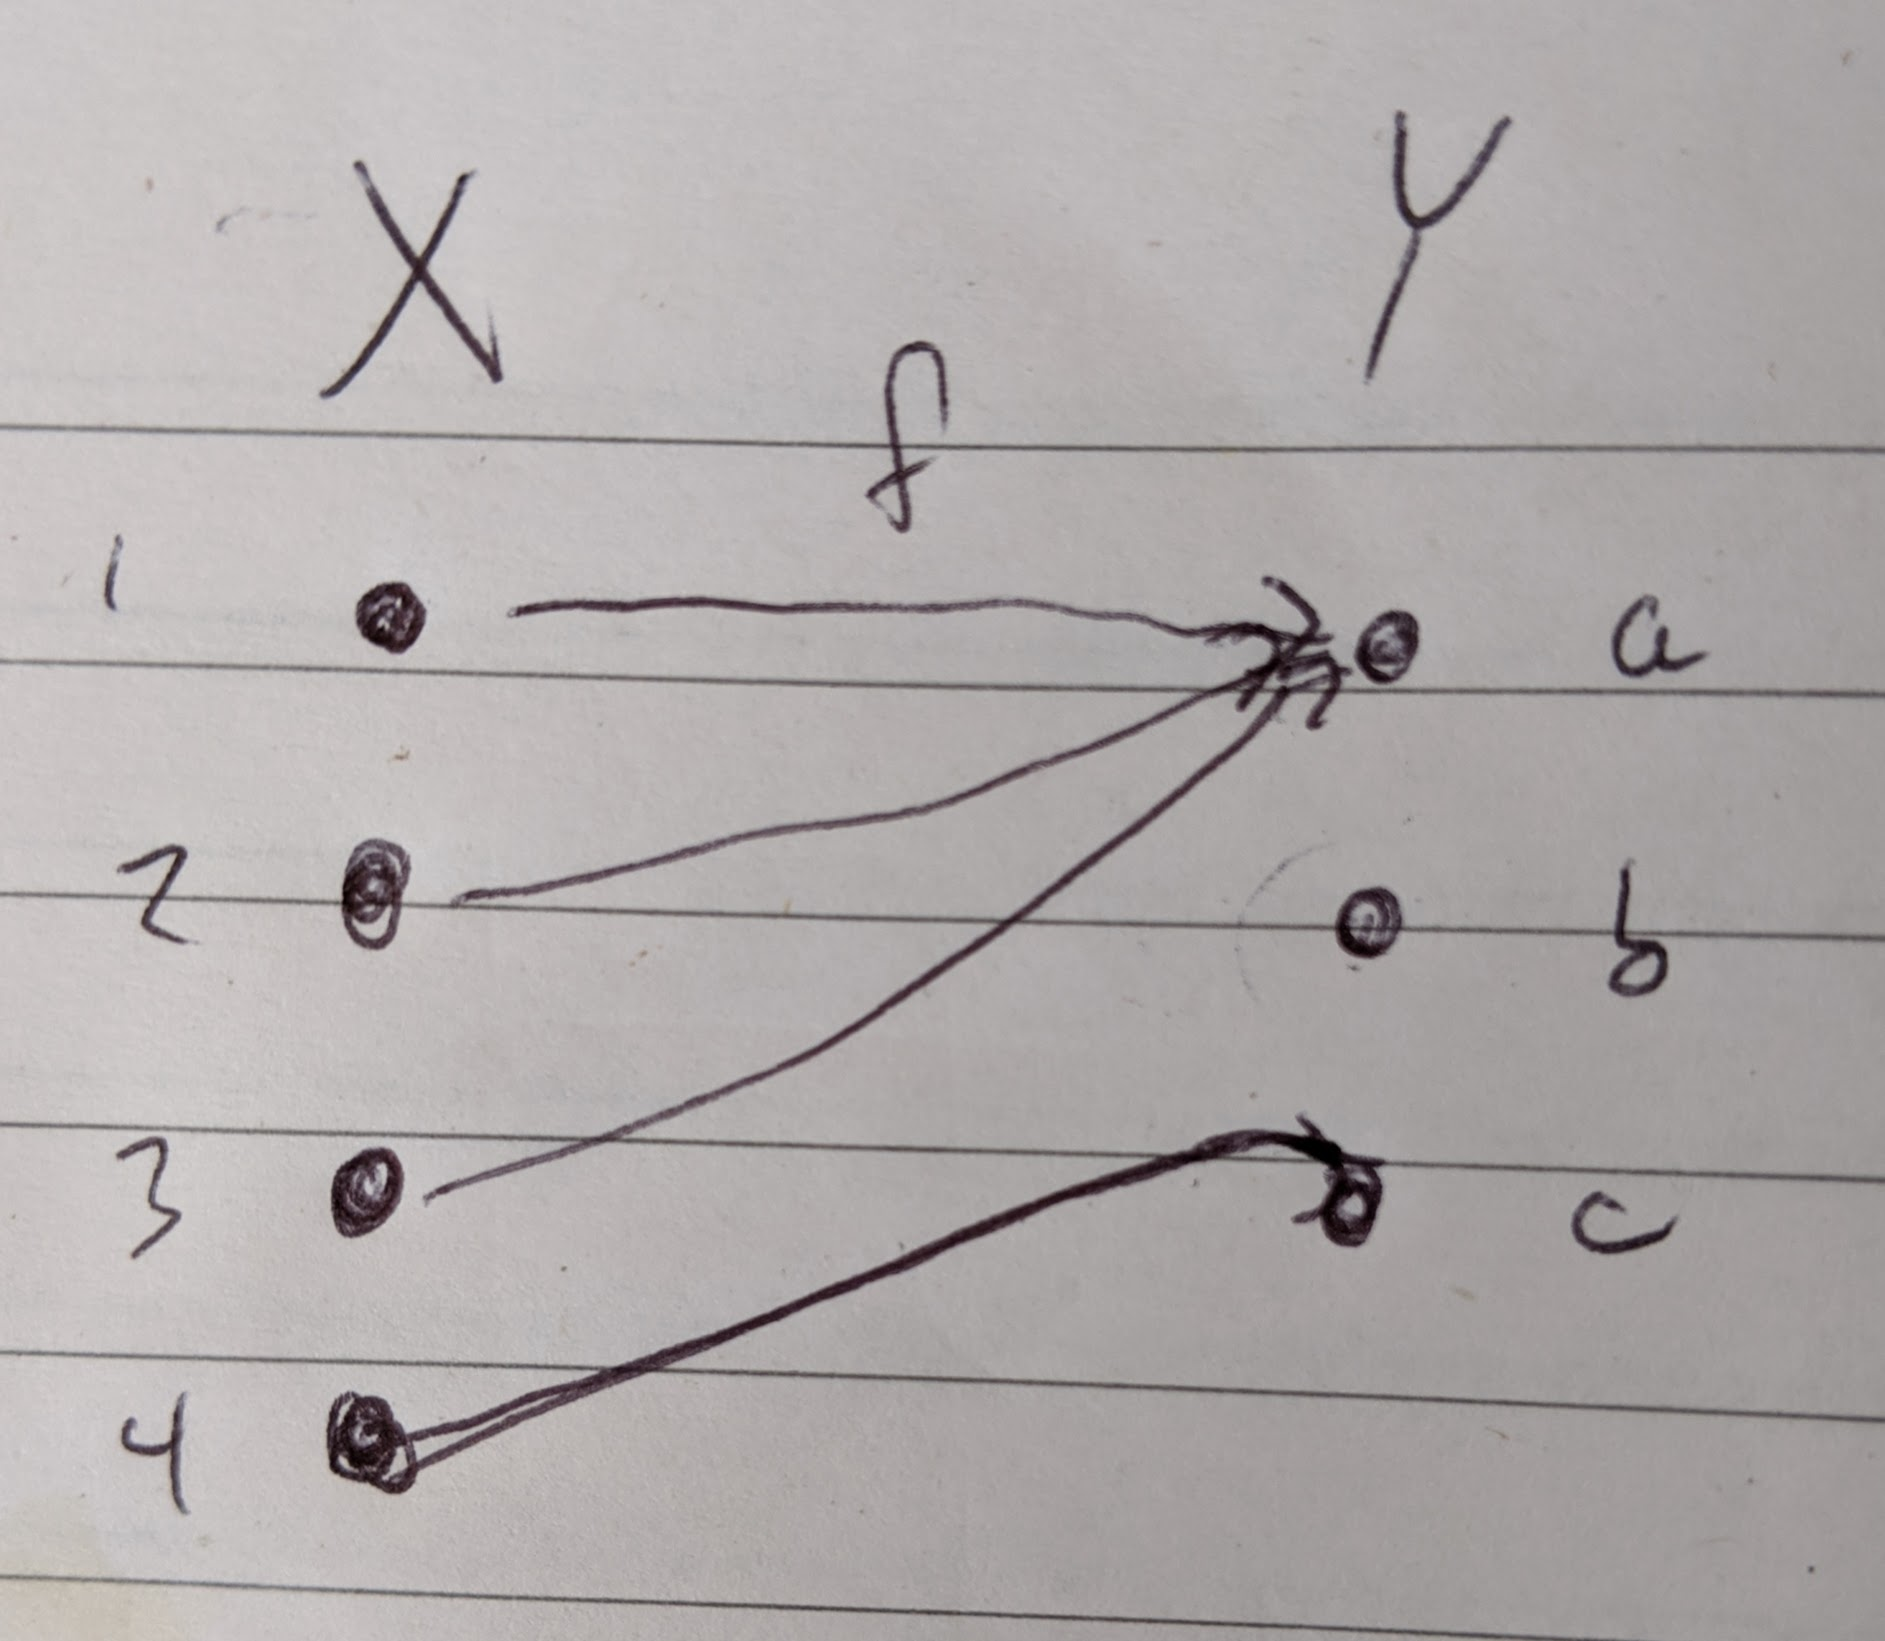
\includegraphics[width=0.5\linewidth]{images/1-118.jpg}
\begin{enumerate}
	\item $f^*(\{a,b\}) = \{1,2,3\}$ and $f^*(\{c\})=\{4\}$
	\item $f_!(\{1,4\}) = \{a,c\}$ and $f_!(\{2,3\})=\{a\}$
	\item $f_*(\{1,4\}) = \{b\}$ and $f_*(\{2,3\})=\{a, b\}$
\end{enumerate}

\exercise{1.119}
Suppose $f$ is left adjoint to $g$.  Show that
\begin{enumerate}
	\item $p\leq (f\fcmp g)(p)$
	\item $(f \fcmp g\fcmp f \fcmp g)(p)\cong (f\fcmp g)(p)$
\end{enumerate}

\solution
\begin{enumerate}
	\item From Proposition 1.107 we immediately have that $p\leq (f\fcmp g)(p)$ from the fact that $f$ is left adjoint to $g$.
	\item If we apply Proposition 1.107 to $(f\fcmp g)(p)\in P$, this gives us $(f\fcmp g)(p)\leq (f\fcmp g)((f\fcmp g)(p))$.  If we apply the other part to $f(p)\in Q$, this gives us $(g\fcmp f)(f(p))\leq f(p)$, and because $g$ is monotone this implies that $(f\fcmp g\fcmp f\fcmp g)(p) \leq (f\fcmp g)(p)$.  Hence $(f \fcmp g\fcmp f \fcmp g)(p)\cong (f\fcmp g)(p)$.
\end{enumerate}

\exercise{1.124, 1.125}
Discussed in person.
